%!TEX root = Thesis.tex

\chapter{Ligand Synthesis and Properties}
\label{ch:ligands}

The xantphos class of diphosphine ligands (Figure \ref{Xantphosligands}) based on a xanthene or xanthene derived backbone are ubiquitous in coordination chemistry and catalysis.  The bis-(diphenylphosphino)xanthene ligands were the first wide bite-angle ligands to be systematically studied for the impact of their bite-angle on catalysis.\cite{Kranenburg1995}  The derivatives showed significant variations in activity and selectivity in the rhodium catalysed hydroformylation of \ce{1-octene}.  Subsequently a large number of derivatives have been reported and they have been studied extensively in different catalytic reactions (for examples see \cite{Kamer2001, Asensio2010, Dieleman2001, Jahromi2012, Birkholz2009, Veen2000b}).  

An important note on nomenclature, the term xantphos is used in the literature to mean either the general class of ligands or the specific ligand 9,9-dimethyl-4,6-bis(diphenylphosphino)xanthene.  For the purposes of this thesis the specific ligand will be referred to as \Phxantphos{} and the term xantphos will be used to represent a generic ligand from this class.  In the literature two different structures are commonly referred to as  \tBuxantphos{}, one with tert-butyl groups on the aromatic backbone and one with tert-butyl groups on the phosphorus atoms.  For the purpose of this thesis the structure with the tert-butyl groups on the phosphorus will be named \tBuxantphos and the structure with the tert-butyl groups on the aromatic backbone will be named \emph{t}-Bu-(\Phxantphos).

\begin{figure}[ht]
\begin{center}
\vspace{0.5cm}
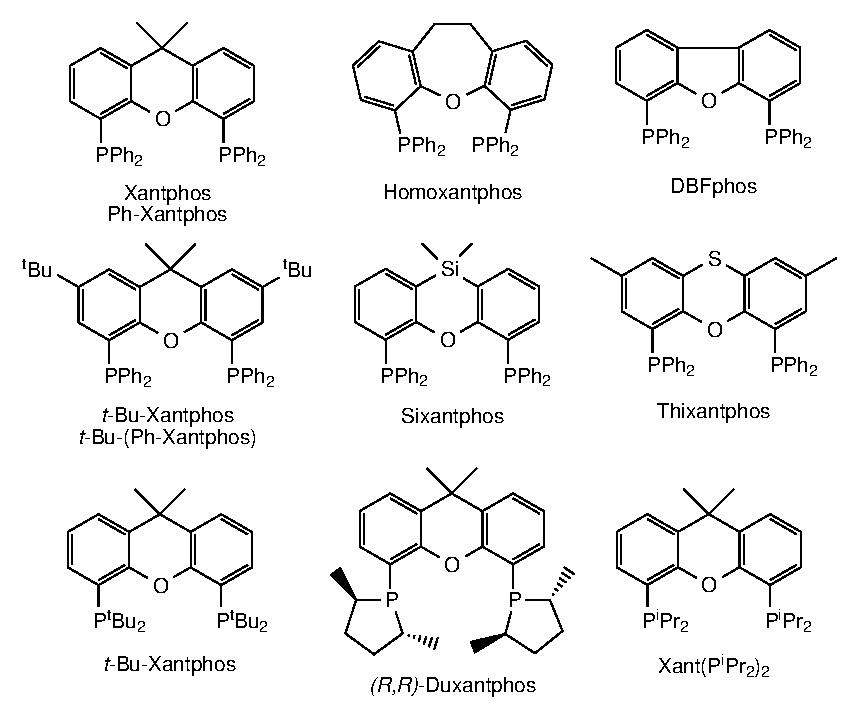
\includegraphics{../Figures/Xantphosligands.eps}
\caption[Examples of the xantphos class of ligands]{Examples of the xantphos class of ligands showing naming and different sites for derivatisation.}
\vspace{0.2cm}
\label{Xantphosligands}
\end{center}
\end{figure}
\vspace{0.2cm}

%A vast number of wide bite-angle ligands based on a xanthene backbone have been synthesised since they were first reported in 1995.\cite{Kranenburg1995, Kamer2001, Esteruelas2011}  The bis-(diphenylphosphino)xanthene ligands were the first wide bite-angle ligands to be systematically studied.  Slight variations in the backbone led to changes in the calculated natural bite-angle.  The derivatives showed significant variations in activity in the rhodium catalysed hydroformylation reacti.  They have since been studied extensively in a range of different reactions \fixme{cite a review or something here} and a number of derivatives have been reported.  

Derivatives of xantphos have focussed mainly on two sites; the bridging group to access a wider range of bite-angles and the phosphine groups.  The phenyl phosphines have been switched for an array for different phosphines including cyclic groups\cite{Veen2000b}, chiral derivatives{\cite{Kamer2001} or changes for solubility.\cite{Buhling1997}  The phosphines have also been switched for different donors including phosphonites,\cite{Dieleman2001} amines, imines, arsines,\cite{Veen2000b} thioethers and others.  Further derivatives with substitutions on the aromatic backbone have also been reported, such as \emph{t}-Bu-(\Phxantphos), or sulfoxantphos\cite{Goedheijt1998} are generally less common as changes here have a limited impact due to their distance from the metal.  

Recently an analogue of xantphos has been reported with sterically bulky tertiary butyl groups on the phosphines (\tBuXantphos, Figure \ref{Xantphosligands}). First reported in 2005 it has been utilised as a ligand in the palladium catalysed cross-coupling of thiols and aryl bromides or triflates\cite{Mispelaere2005}, the ligand has since been tested for activity in platinum-catalyzed amination of allylic alcohols\cite{Ohshima2009} and the iron catalysed sp$^3$-sp$^3$ cross-coupling reactions of alkyl halides and alkyl Grignard reagents.\cite{Dongol2007}  However, in each of these cases the complexes were presumed to be formed in the catalytic mixture and were not characterised.  

To date, the only characterised transition metal complexes of \tBuxantphos{} are the series of gold halide complexes [(\tBuxantphos)\ce{Au][AuX2]} where X = Cl$^-$, Br$^-$ or I$^-$.\cite{Partyka2010}  In these structures the \tBuxantphos{} complexes were shown to have large bite angles of 143.0, 142.5 and 143.0\degrees{} for Cl$^-$, Br$^-$ and I$^-$ respectively.  When the same reaction was attempted with the Ph-xantphos ligands, complexes of the type \ce{[(Xantphos)(AuX)2]} were formed.\cite{Pintado2004, Partyka2010}  These structures clearly indicate the difference between the phenyl and \tBu{} substituted xantphos ligands and the significant impact of the increased steric bulk of the \tBu{} groups on the bonding mode of the ligands.  

The xantphos system is also interesting as there is the potential for different bonding modes.  The most common is the \emph{cis}-bidentate chelate, although a \emph{trans}-bidentate chelate has been reported.  A third mode where the oxygen bridge coordinates to the metal centre in addition to the phosphines is also possible.  A limited number of examples of this type of coordination exist either with xantphos itself or with derivatives.\cite{Asensio2010, Esteruelas2011, Esteruelas2013, Alos2013}\fixme{Get relative numbers of crystal structures or something from CCDC}.  The potential for coordination of the oxygen offers the ability to stabilise intermediates and transition states in catalytic reactions allowing for increased reactivity or selectivity.

\begin{figure}[ht]
\begin{center}
\vspace{0.5cm}
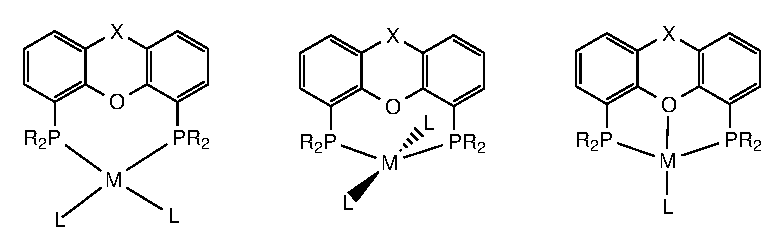
\includegraphics{../Figures/Bondingmodes.eps}
\caption[Different bonding modes of xantphos ligands]{Different bonding modes of xantphos ligands}
\vspace{0.2cm}
\label{Bondingmodes}
\end{center}
\end{figure}
\vspace{0.2cm}

The xantphos ligands are widely used in catalysis but \tBuxantphos{} has shown little activity.  This is an indication that the chemistry of the two complexes is substantially different as shown by the only characterised complexes of \tBuxantphos{} reported.  Due to this difference in behaviour further explorations into the coordination activity of \tBuxantphos{} and the reasons for this difference was deemed to be of scientific interest.

%As these gold complexes are the only examples of characterised tBu-xantphos metal complexes and the phenyl xantphos ligands are so widely utilised the tBu-xantphos ligand system was chosen for further study.  

\section{Ligand Synthesis}\label{section:ligandsynthesis}

In 2002 van Leeuwen et al. reported their unsuccessful attempts to synthese \emph{t}-Bu-xantphos from either the dilithiated backbone or starting with 9,9-dimethyl-4,5-bis(dichlorophosphino)xanthene, suggesting that steric crowding from having two \emph{tert}-butyl groups on a single phosphorus prevented the successful coupling.\cite{Zuideveld2002}  However, in 2005 a synthesis of \emph{t}-Bu-xantphos from the dilithiated backbone was reported.\cite{Mispelaere2005}  This synthesis involved attack on the lithiated backbone by chlorodi-\emph{t}-butylphosphine at 60 \degC{} for 24 hours, generating the product in 38\% isolated yield.

%The previously reported synthesis for tBu-xantphos\cite{Mispelaere2005} involved lithiation of the backbone in heptane followed by the addition of chlorodi-\emph{tert}-butyl phosphine and heating to 60\degrees C for 24 hours.  The reportedly air-stable product was obtained and recrystallised from n-propanol in 38\% yield.  Attempts to use this method for the synthesis of tBu-thixantphos yielded a mixture of products.\fixme{check this}

Attempts to utilise the synthesis method of \tBuxantphos{} to synthesise \tButhixantphos{} resulted in a number of products which were unable to be identified.  An alternative method using a potassium \emph{tert}-butoxide and \emph{n}-butyllithium ``superbase'' formed a mixture of products from which separation attempts were unsuccessful.  This superbase results in significant amounts of organopotassium compounds which are more active metallating agents.  However, organopotassium compounds are also more active in cleavage of ethers.\cite{Bhatt1983}  Hence the mixture of products, may result from cleavage of the ether or thioether bridges resulting in undesired compounds.

%This reference doesn't actually cover organopotassium, just sodium and lithium.

The synthesis of tBu-thixantphos was attempted using the initially reported synthesis of xantphos\cite{Kranenburg1995} (Scheme \ref{Ligandsynthesis}).  This method involves the dilithiation of the backbone using \emph{sec}-butyllithium and \gls{TMEDA} followed by reaction with chlorodi-\emph{tert}-butyl phosphine.  The reaction required extended periods and was allowed to proceed until no further change was determined by NMR (typically 7 days).  This reaction resulted in a mixture of the mono and diphosphine.  The diphosphine was isolated as white crystals by recrystallisation from \emph{n}-propanol.  The remaining \emph{n}-propanol solution of the monophosphine could be reduced to dryness and then reused for a second lithiation and reaction with chlorodi-\emph{tert}-butyl phosphine to produce more of the desired diphosphine.  

 %carried out in diethyl ether with \gls{TMEDA} using \emph{sec}-butyllithium, added at -78\degrees C followed by addition of the chlorodi-\emph{tert}-butyl phosphine and stirring for 16 hours.  After 16 hours of reaction the NMR spectra showed a mixture of mono and di-substituted products.  The reaction was allowed to proceed until no further change was determined by NMR (typically 7 days).  The reaction invariably produced a mixture of mono and diphosphine.  The diphosphine was separated from the monophosphine by-product by recrystallisation from hot n-propanol and cooling at -16\degC.  The diphosphine was obtained in \fixme{yield} as white crystals.  

\begin{scheme}[ht]
\begin{center}
\vspace{0.5cm}
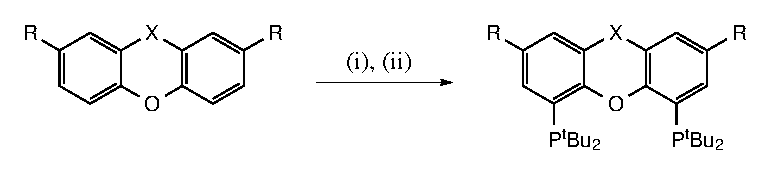
\includegraphics{../Schemes/Ligandsynthesis.eps}
\caption[Ligand synthesis]{Synthesis of \tBuxantphos{} (X = \ce{CMe2}, R = H), \tButhixantphos{} (X = S, R = Me) and \tBusixantphos{} (X = \ce{SiMe2}, R = H).  \emph{i}: \emph{s}-BuLi, \ce{Et2O}. \emph{ii}: \ce{ClPtBu2}}
\vspace{0.2cm}
\label{Ligandsynthesis}
\end{center}
\end{scheme}
\vspace{0.2cm}

The steric bulk of the tertiary butyl groups leads to difficulties in the synthesis.  Reaction with one equivalent of chlorodi-\emph{tert}-butyl phosphine to form the monophosphine is clean and rapid, occurring overnight.  However, the steric bulk of the monophosphine results in a much slower second addition, requiring extended reaction times to allow for significant conversion.  When the reaction is allowed to proceed for longer than one week no additional conversion is observed.  This is likely the result of degradation of either the lithiated monophosphine or the \emph{sec}-butyllithium before the second lithiation can occur.  Over extended periods organolithium reagents cleave diethyl ether resulting in alkanes, alkenes and lithium ethoxide (Scheme \ref{Organolithium}).\cite{Bhatt1983, Gilman1954}  \emph{sec}-butyllithium has been shown to completely react with diethyl ether in one day.\cite{Gilman1954}  Although the reaction between diethyl ether and aryllithium is slower (half-time of 100 hours), the extended reaction periods required for the second phosphine addition mean that this may play a significant role.  \fixme{the 100 hrs is from Schlosser's book (organometallics in organic synthesis), check that it is correct and then reference}

%Between \emph{n}-butyllithium the reaction occurs with a half time of 6 days at 25\degC{}.\fixme{ref}  Although an aryl lithium with an ortho oxygen group would be expected to reaction more slowly with the diethyl ether this is one possible pathway for reaction.  \fixme{does this happen in THF}  

%This is likely a result of the steric bulk of the \emph{tert}-butyl groups hindering the second addition reaction.  However, over time organolithium reagents react with diethyl ether generating lithium ethoxide and ethene (Scheme \ref{Organolithium}).  This reaction occurs with a half time of 6 days at 25\degC{} for \emph{n}-butyllithium.  This is likely the reason for the lack of observed reaction after periods of one week.

\begin{scheme}[ht]
\begin{center}
\vspace{0.5cm}

\includegraphics{../Schemes/Organolithium.eps}
\caption[Reaction of n-butyllithium with diethyl ether]{Reaction of n-butyllithium with diethyl ether}
\vspace{0.2cm}
\label{Organolithium}
\end{center}
\end{scheme}
\vspace{0.2cm}

In order to promote the dilithiation a preformed sec-butyllithium, \gls{TMEDA} complex was added to a solution of the backbone.  An initial colour change to yellow (\tButhixantphos{} and \tBusixantphos) or green (\tBuxantphos) was observed, indicative of monolithiation.  After stirring overnight this changed to red or yellow respectively.  This colour change gives a clear indication of successful dilithiation.  In order to favour the diphosphine over the monophosphine the lithiated backbone was then added slowly to an ethereal solution of chloro-di-tert-butyl phosphine.  Although a mixture of the mono- and diphosphine was always obtained this order of addition was found to be more successful, resulting in increased yields.

The \tBuxantphos{} ligand obtained using our method had \proton{} and \carbon{} NMR spectra consistent with the literature.\cite{Mispelaere2005} However the \phosphorus{} chemical shift differed by 2.2~ppm (10.2~ppm in this study compared to 12.4).  The NMR spectra for the reported and the synthesised samples were both obtained in \ce{CDCl3} and referenced to an external 85\% \ce{H3PO4} standard.  Hence the reason for this difference is unclear.  However, as the remainder of the NMR and other characterisation data is consistent, it is likely that the two compounds are identical and a typographical error or otherwise was made in the preparation of the earlier paper.

The synthesis of these ligands utilises directed ortho metallation as first described independently by Gilman and Wittig in 1939 and 1940 respectively.\cite{Gilman1939, Wittig1940} Directed ortho metallation uses a heteroatom which coordinated to the organolithium thereby directing it to the ortho sites.  In this case the ether linkage can act as a director for the lithiation.  Once lithiated the electron density on the oxygen stabilises the lithiated site against degradation.  For \tBuxantphos{} and \tBusixantphos{} the oxygen is the only atom present with lone pairs of electrons and thus the lithiation occurs exclusively in the desired positions ortho to the oxygen.  However, phenoxathiin has both an ether and a thioether which can both act as ortho directors.\cite{Organolithiummethods}  Previous research shows that in the presence of both ether and thioether groups the lithiation will occur ortho to the oxygen.\cite{Turck1997}  However, once the first lithiation has taken place the oxygen is unable to contribute significantly to the second lithiation.  For \tBuxantphos{} and \tBusixantphos{} the influence of the oxygen is still sufficient that the second lithiation occurs in the other ortho position.  However for phenoxathiin the thioether acts as a second directing group and the lithiation occurs ortho to the sulfur.  Resulting in the undesired product \fixme{reference to trans ligand}.  The addition of methyl groups meta to the thioether provides sufficient steric hindrance that the second lithiation also occurs ortho to the oxygen and the desired \tButhixantphos{} is produced.  

%The methyl groups on the aromatic system of \tButhixantphos{} was found to be important.  The attempted synthesis of a \tButhixantphos{} without methyl groups resulted in substitution ortho to the oxygen and ortho to the sulfur in a transoid configuration (Scheme \ref{Transthixantphos}).  It is likely that using three equivalents of \emph{sec}-butyllithium results in lithiation in three positions, the two ortho to the oxygen and one ortho to the sulfur.  The first addition of phosphine attacks one ortho to the oxygen.  This creates increased steric hindrance at the second site ortho to oxygen so the second equivalent of phosphine preferentially attacks in the least hindered site; ortho to the sulfur.  \fixme{this paragraph may in fact just be lies}.  The oxygen in the bridge of all three ligands acts as a directing group to promote lithiation in the ortho position.  However in the case of \tButhixantphos{} the sulfur can also act as a directing group (though less strongly that the oxygen) this leads to competition for the lithiation site and requires the methyl on the backbone to provide steric hindrance and prevent lithiation ortho to the sulfur.  This difficulty was not encountered with either the \tBuxantphos{} or \tBusixantphos{} ligands.  The carbon and silicon groups are not able to interact with the lithium and promote ortho lithiation so the lithiation occurs exclusively ortho to the oxygen. \fixme{see directed ortho lithiation for more info}

\begin{scheme}[ht]
\begin{center}
\vspace{0.5cm}
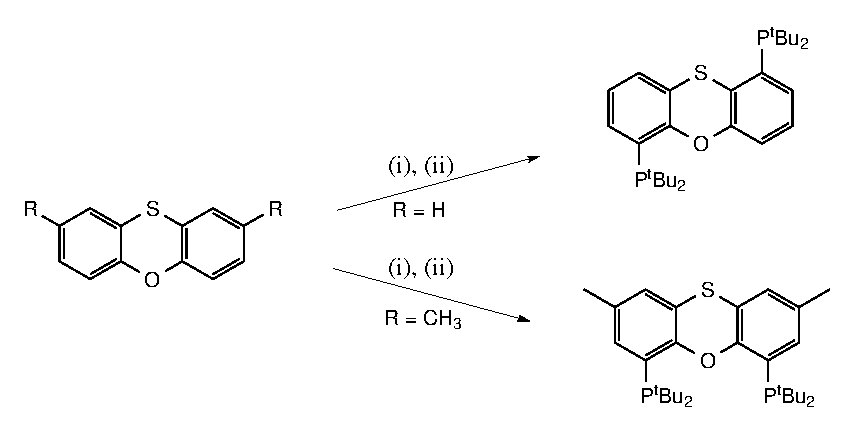
\includegraphics{../Schemes/Transthixantphos2.eps}
\caption[Influence of methyl groups on the synthesis of \tButhixantphos]{Influence of methyl groups on the synthesis of \tButhixantphos. \emph{i}: \emph{sec}-BuLi, \ce{Et2O}. \emph{ii}: \ce{ClPtBu2}}
\vspace{0.2cm}
\label{Transthixantphos}
\end{center}
\end{scheme}
\vspace{0.2cm}


However, the synthesis of \tBusixantphos{} was not problem free.  Given the extended reaction times necessary to obtain the diphosphines, the formed diphosphine is in solution with large volumes of lithium chloride for a substantial amount of time.  NMR analysis of the synthesis of \tBusixantphos{} showed the formation of a significant amount of a compound with a single peak in the \phosphorus{} NMR spectrum at 15 ppm.  No new peaks were observed in the \proton{} NMR spectrum.  However, due to the similarity in the spectra to those of \tBusixantphos H+ we propose that this compound is [Li\tBusixantphos]Cl.  The compound is unchanged through extensive water washing.  Attempts to remove the lithium ion using the lithium specific chelating agent, 12-crown-4, were unsuccessful.  Reaction with tetrafluoroboric acid in order to exchange the lithium for a proton led to the formation of a new species the nature of which could not be determined.  The formation of [Li\tBusixantphos]Cl results in a significant loss of product for the synthesis of \tBusixantphos{} resulting in lower yields than those for \tBuxantphos{} and \tButhixantphos{}.

%It was found the \tBusixantphos{} tended to capture lithium ions between the two phosphorus atoms.  These lithium ions were tightly bound and were retained through several cycles of washing with water.  The nature of this species was confirmed by reaction with a sample of the pure ligand with lithium chloride, resulting in the same product.  \fixme{do this} Attempts to react the lithiated \tBusixantphos{} with tetrafluoroboric acid to exchange the lithium ion for a proton was unsuccessful and instead resulted in possibly a boron trifluoride bound between the two phosphines.\fixme{check this with boron NMR etc.}  Attempts to remove the lithium using the lithium specific chelating agent, 12-crown-4, were unsuccessful.  Due to the inability to remove the lithium this represents a source of significant loss of product for the synthesis of \tBusixantphos{} resulting in lower yields than those for \tBuxantphos{} and \tButhixantphos{}.

The NMR data of the newly reported \tButhixantphos{} and \tBusixantphos{} ligands are consistent with expectations (Table \ref{table:ligandNMRdata}).  In both cases a plane of symmetry reduces the number of signals hence showing a single peak in the \phosphorus{} NMR.  The \phosphorus{} chemical shift for \tBuxantphos{} synthesised in this work is 10.2 which differs from the reported value of 12.4\cite{Mispelaere2005}, however the \proton{} and \carbon{} data is consistent.  


\begin{table}[ht]
\small
\caption[Selected NMR Data for Xantphos Ligands]{Selected NMR Data for Xantphos Ligands in \ce{CDCl3}}
\vspace{1em}
\label{table:ligandNMRdata}
\begin{center}
\begin{tabular}{l c c c c c c}
	\toprule
	~\bfseries{Diphosphine} & \bfseries{$\delta$P (ppm)} & \multicolumn{5}{c}{\bfseries{$\delta$H (ppm)}} \\
	\midrule		
	~\tBuXantphos\cite{Mispelaere2005}	& 12.4 & 1.21-1.26 & 1.57 s & 7.02 t & 7.38 dd & 7.60 d\\
	~\tBuXantphos{}(This work) 		& 10.2 & 1.21-1.25 & 1.57 s & 7.03 t & 7.38 dd & 7.60 d\\
	~\tBuThixantphos				& 9.5 & 1.22-1.24 & 2.25 s & 6.88 s & 7.29 s & \\
	~\tBuSixantphos				& 8.42 & 1.29 vt & 0.46 s & 7.12 t & 7.53 d & 7.87 d\\ 
	\bottomrule{}
\end{tabular}
\end{center}
\end{table}

The \proton{} NMR data for the \tBuxantphos{} ligands show a \ce{X18A}A'\ce{X18}' spin system for the \emph{tert}-butyl protons.  For a system where the two A atoms (in this case the phosphorus) are strongly coupled this leads to a difference of zero between the three and five bond couplings (e.g. when the phosphorus atoms are in a trans configuration in a metal complex) resulting in a virtual triplet.  However, in this case there is no atom between the phosphorus atoms so we would expect a three-bond and a nine-bond coupling.  A nine-bond coupling is an extremely remote coupling which we would expect to be negligible.  Based on previous reports\cite{Harris1964, Abraham1961} this peak shape with two sharp outer lines and a broad inner peak occurs with the difference between the short and long range couplings is very small but not zero.  For this to occur the phosphines must have some degree of through-space spin-spin coupling through their lone pairs of electrons (for a review of nonbonded spin-spin coupling see Hierso\cite{Hierso2014}).  This is further supported by the difference in the \proton{} spectra for the three ligands; the central peak is sharpest for \tBusixantphos{} then \tButhixantphos{}.  For \tBuxantphos{} some further detail can be seen indicating that this has the weakest through space coupling.  This trend is consistent with the expected changes in the distance between the phosphines upon changing the backbone which will impact the degree of through-space coupling that can occur and therefore the difference in the short and long-range coupling constants.

%include spectra showing the tBu peak?

\section{Bite Angle Calculations}

The steric and electronic properties of diphosphine ligands determine their complexation behaviour with transition metals and can influence the reactivity of the complex particularly impacting the activity and selectivity in catalytic transformations.\cite{Freixa2003, Birkholz2009}  The xantphos class of ligands were initially investigated as ligands with consistent electronic properties and steric bulk so that the impact of the bite-angle on rhodium catalysed hydroformylation could be studied exclusively.\cite{Kranenburg1995}  Consequently a number of studies have investigated the bite-angle impact on a variety of catalytic conversions (for examples see\cite{Kranenburg1995b, Haaren2001b, Dudle2011b, Fanjul2013, Birkholz2009}).  The bite-angle is a result of both the steric and electronic properties of the ligand.\cite{Freixa2003}

The natural bite-angle (\natbiteangle) was first described by Casey and Whiteker\cite{Casey1990} as a theoretically determined parameter to indicate the preferred chelation angle of diphosphine ligands irrespective of the metal they are coordinating to.  Computationally these are calculated using a dummy atom at 2.3 \si{\angstrom} in the place of a metal and optimising the geometry of the ligand system, the natural bite-angle can then be measured.  This is often used in combination with a flexibility range (the bite-angles that can be obtained within a range of 12.6~\si{\kilo\joule\per\mol}).  

In order to determine the usefulness of the natural bite-angle in determining the coordination bite-angle an investigation into this using data from the Cambridge Crystallographic Data Centre was performed.  The results are summarised in Table \ref{table:biteangles} which is sorted by the natural bite-angle.  The natural and median experimental bite-angles show a good correlation described by the equation $experimental = 1.1013$\natbiteangle $- 5.6972$, ($R^2 = 0.9246$).  Some of the experimental and natural bite-angles that are most relevant to this work show significant differences (for example \tBuxantphos{} \natbiteangle{} = 140\degrees, experimental = 153.317\degrees and \Phsixantphos{} \natbiteangle{} = 109, experimental = 99.165\degrees) this may be due to the low numbers of structures for these ligands (4 and 5 respectively) at which point the metals used will have a significant impact. 

\begin{table}[ht]
\small
\caption[Bite-angles for a range of diphosphine ligands]{Bite-angles for a range of diphosphine ligands taken from the Cambridge Crystallographic Database} 
\vspace{1em}
\label{table:biteangles}
\begin{center}
\begin{tabular}{c c c c c c}
	\toprule
	~~\bfseries{Diphosphine}~~ & \bfseries{Total Structures} & \bfseries{P-P ($\si{\angstrom}$)} & \bfseries{Range (\degrees)} & \bfseries{Bite-Angle (\degrees)} & \bfseries{$\beta$\sub{n} (\degrees)}\\
	\midrule
	 ~dppm			& 384	& 2.718	& 62.757 - 77.706 	& 71.062 	& 73	\\
	 ~dppe			& 1939	& 3.095	& 71.073 - 92.926	& 83.818	& 78 \\
	 ~dppp			& 3237	& 3.308	& 83.333 - 105.420	& 92.181	& 86 \\ 
	~BINAP			& 146	& 3.296	& 85.9820 - 115.666	& 91.925	& 92 \\
	~dppb			& 127	& 3.391	& 89.447 - 111.491	& 94.240	& 99 \\
	 ~DPEphos		& 101	& 3.844	& 96.094 - 158.531	& 112.691	& 102 \\
	 ~\PhXantphos		& 65		& 3.908	& 98.829 - 153.134	& 108.535	& 111 \\
	 ~BISBI			& 4		& 4.079	& 103.533 - 151.951	& 124.789 & 123 \\
	~Ph-sixantphos		& 5		& 3.691 	& 95.250 - 152.149	& 99.165 & 109 \\
	~Ph-thixantphos	& 3		& 4.021	& 109.528 - 155.050	& 111.724	& 110 \\
	~tBu-xantphos		& 4		& 4.527	& 152.302 - 153.456 & 153.317 & 140 \\
	~dpp-benzene		& 116	& 3.101	& 74.380 - 92.499	& 84.900	& 83\\
	~dppn			& 25		& 3.176	& 79.867 - 93.270	& 86.864	& 82 \\
	~dppx			& 19		& 3.569	& 90.045 - 106.186	& 102.636	& 90 \\
	~dbpe			& 109	& 3.200	& 83.989 - 95.949	& 90.369	& 87	\\
	~dbpp			& 12		& 3.503	& 94.556 - 104.857	& 99.175	& 99	\\
	~dbpx			& 10		& 3.634	& 98.758 - 107.255	& 101.881	& 101 \\
	\bottomrule{}
\end{tabular}
\end{center}
\end{table}

%\begin{figure}[ht]
%\begin{center}
%\vspace{0.5cm}
%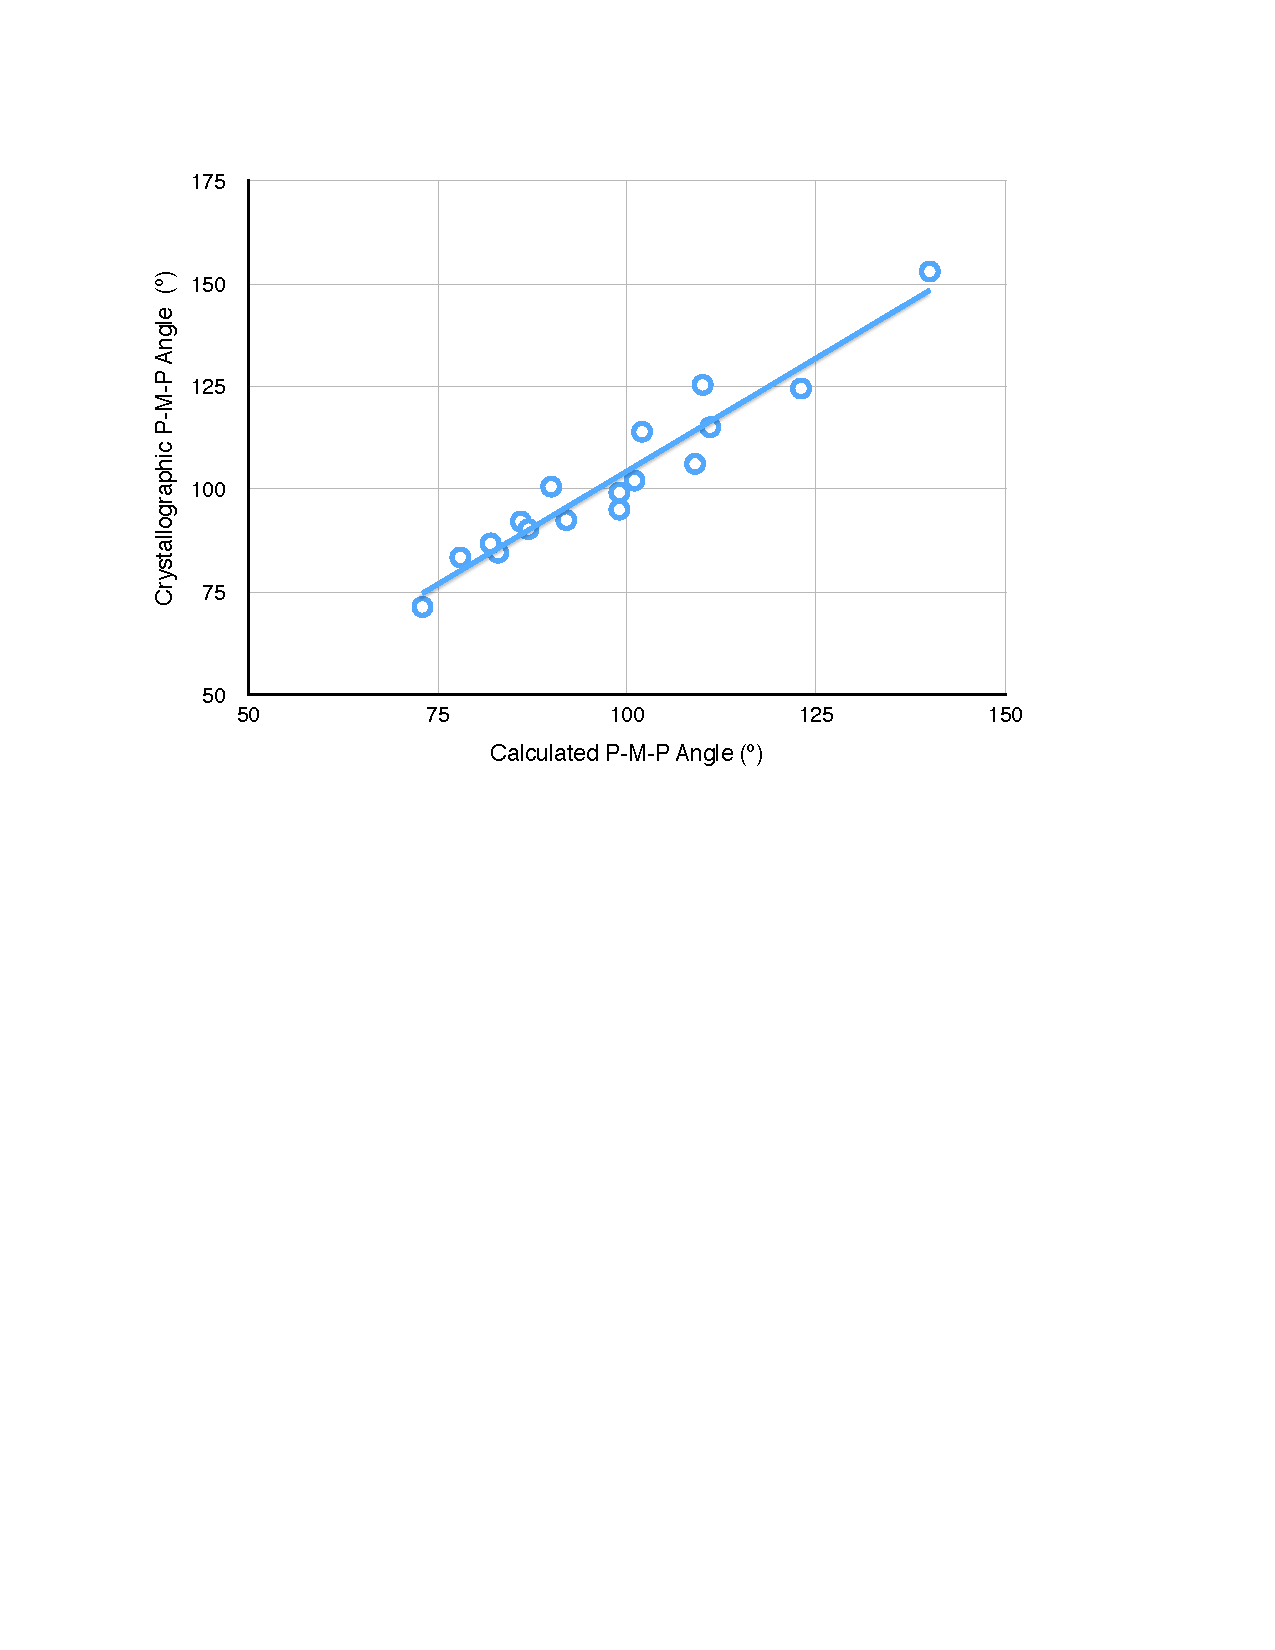
\includegraphics[scale=0.8]{../Figures/Bite-anglegraph}
%\caption[Comparison of the Natural Bite-Angle with the Experimentally Determined Bite-Angle]{Comparison of the Natural Bite-Angle with the Experimentally Determined Bite-Angle.  Trendline $ y = 1.1013x - 5.6972$, Linear regression $R^2 = 0.9246$}
%\vspace{0.2cm}
%\label{Biteanglegraph}
%\end{center}
%\end{figure}
%\vspace{0.2cm}

In order to determine the potential differences between \tBuxantphos{} and \Phxantphos{} the natural bite-angles for the three \tBu{} ligands were calculated.  Bite-angle calculations are typically carried out using molecular mechanics, in this study we used a density functional theory instead, we thus calculated the natural bite-angles of the previously reported bite-angles for the \Phxantphos{} series of ligands and \tBuxantphos{} (Table \ref{table:biteanglescalculated}).  These show good agreement with those calculated using molecular mechanics.  Given the good agreement of our DFT obtained values and the literature values we continued by calculating the bite-angles for the two new ligands \tButhixantphos{} and \tBusixantphos{}.  A number of different bite-angles have been reported for the \Phxantphos{} series, due to different computational set-ups.  

\begin{table}[ht]
\small
\caption[Bite angles of xantphos ligands]{Bite angles of xantphos ligands}
\vspace{1em}
\label{table:biteanglescalculated}
\begin{center}
\begin{tabular}{c c c c}
	\toprule
	~\bfseries{Diphosphine}	&\bfseries{Molecular Mechanics (\degrees)}&\bfseries{Reference}	&\bfseries{DFT (\degrees)}\\
	\midrule		
	~\PhXantphos		~~&~108, 111.7~~	& ~\cite{Birkholz2009}	&~~118.59~~	\\	
	~\PhThixantphos	~~&~110, 109.4~~	& ~\cite{Birkholz2009, Kranenburg1995}&~~118.04~~	\\
	~\PhSixantphos	~~&~108, 108.7~~	& ~\cite{Birkholz2009, Kranenburg1995}&~~111.43~~	\\
	~\tBuXantphos		~~&~140~~		&~\cite{Birkholz2009}~~	&~~159.93~~	\\
	~\tBuThixantphos	~~&~~~			&~~~~			&~~126.98~~	\\
	~\tBuSixantphos	~~&~~~			&~~~~			&~~126.80~~	\\
	\bottomrule{}
\end{tabular}
\end{center}
\end{table}

%  including allylic alkylations\cite{Haaren1999}, rhenium catalysed hydrogenation\cite{Dudle2011b} and the palladium catalysed hydromethoxycarbonylation of ethene.\cite{Fanjul2013}  
%reviews have investigated whether the bite-angle impact is 

The natural bite-angles for the \tBuxantphos{} series of ligands are much larger than for the phenyl substituted ligands.  Given that the remainder of the ligands is unchanged this effect is due to the impact of the \tBu-groups.  These groups are more electron donating than the phenyls so may result in more electron density on the phosphorus atoms resulting in an electrostatic repulsion of the two phosphorus atoms.  The \tBu-groups have a larger steric impact than the planar phenyl rings.  This would result in a larger bite-angle as the steric bulk of the \tBu substituents pushes the two phosphines further apart.  The trend between the two groups is the same with the carbon bridged having the largest \biteangle{} and the silicon bridged having the smallest.

The bite-angles of the \tBuxantphos{} ligands is likely to have a significant impact on their coordination chemistry.  The phenyl ligands form a range of complexes favouring \cis-chelation in square-planar and octahedral complexes, although \emph{trans} square planar complexes have been reported\cite{Petocz2004}.  With bite-angles of 128-142\degrees{} the ligands will likely prefer trigonal planar coordination environments close to 120\degrees.  However the \biteangle s are halfway between the \cis and \trans coordination angles for square planar and octahedral complexes which may result in mixtures of products.  The ratio between the two geometries may change depending on which ligand is used with \tBusixantphos{} favouring \cis-coordination while \tBuxantphos{} favours the \trans-coodination.  The \tBu-groups are very sterically demanding and \cis-coordination of \tBu substituted phosphines is rare\fixme{citation, scifinder or CCD} so this may push the ligands to prefer \trans-coordination modes.

Diphosphine ligands that exhibit exclusive \trans-chelation have been described in a review as elusive.\cite{Freixa2008}  \PhXantphos{} itself can form \trans-chelates\cite{Petocz2004}, however these form as a mixture of the \cis and \trans isomers rather than forming as the pure \trans isomer.  Only a small number of these \trans-chelates for \Phxantphos{} have been reported compared to the majority of complexes where the \cis-chelate forms.  A limited number of ligands exist that can form \trans-chelates, however, rarer are those that do not form \cis-chelates and rarer still are the truly \trans-chelating ligands with a bite-angle of 180\degrees{} and an undistorted coordination plane. 

The wide bite-angles of these ligands may also result in interesting catalytic activity.  Previously reported uses of \tBuxantphos{} have added the ligand to a metal precusor and formed the catalyst in situ.  However platinum, palladium and iron prefer either square-planar or octahedral coordination and if the \tBuxantphos{} ligand coordinated in a \trans configuration this may prevent the oxidative addition or reductive elimination of other ligands.  Hence although \tBuxantphos{} has not shown activity in catalytic systems to date, these ligands may find more use in systems with less rigid metals such as silver or in rhodium catalysed hydroformylation.

\section{Oxidation}

Although previous literature reports \tBuxantphos\cite{Mispelaere2005} as an air-stable solid, this was not the case for at least \tButhixantphos.  The ligands are resistant to oxidation and can be handled in the air for short periods.  However, storage in the air leads to slow oxidation.  

The ligands appear to be more stable to oxidation using hydrogen peroxide than \Phxantphos{}.  Although the \tBuxantphos{} ligands oxidise slowly in the air which \Phxantphos{} does not; attempts to directly oxidise using a large excess of hydrogen peroxide in acetone requires extended periods of reflux while \Phxantphos{} undergoes complete oxidation after only 1 hour at room temperature.\cite{Jahromi2012}

%However problems were encountered with this as the thioether bridge is also susceptible to oxidation.  As such attempts to oxidise the phosphines of \tButhixantphos resulted in oxidation of one of the phosphine arms and the thioether bridge to a sulfoxide or sulfone resulting in a mixture of products.  

\section{Basicity}

As discovered during the synthesis of \tBusixantphos{} the ligands have the ability to coordinate small cations.  Although only \tBusixantphos{} coordinated lithium to any significant degree during the synthesis, all three of the ligands are significantly acid sensitive and will react with any adventitious proton source resulting in the protonation at one of the phosphines.  Although stable for short periods in deutero-chloroform, over time chloroform produces hydrochloric acid \emph{via} photo-degradation which readily protonates the ligands

The phosphonium salts can be prepared directly by reaction with either \ce{CHPh(SO2CF3)2} (\pKa = 2.0 in DMSO) or \ce{CH2(SO2CF3)2} (\pKa = 2.4 in DMSO) resulted in the phosphonium ions \fixme{compound reference}, Scheme \ref{Protonation}.  These acids are useful as they are non-hygroscopic solids allowing for accurate stoichiometry.  The phosphonium salts formed all display a single peaks in the \phosphorus{} NMR spectrum ($\Delta\delta$ = 5.9 - 7.2) and half the expected signals in the \proton{} NMR spectrum.  This indicates a rapid exchange of the proton between the two phosphorus atoms.

\begin{scheme}[ht]
\begin{center}
\vspace{0.5cm}
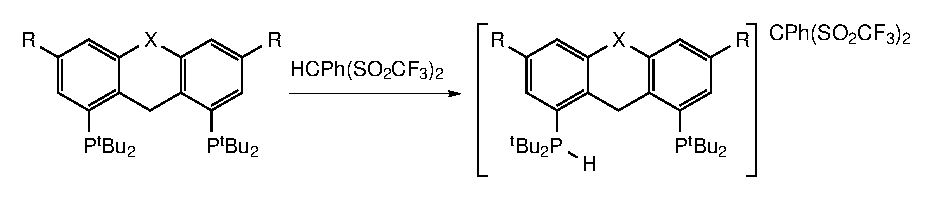
\includegraphics{../Schemes/Protonation.eps}
\caption[Protonation of the ligands using a strong acid]{Protonation of the ligands using a strong acid}
\label{Protonation}
\end{center}
\end{scheme}
\vspace{0.2cm}

The difference in the rate of exchange of the proton in the three compounds in clearly shown by the \phosphorus{} and \proton{} NMR spectra.  The \phosphorus{} NMR signal is sharpest for \tBusixantphos{} followed by \tButhixantphos while \tBuxantphos has a very broad signal.  Indicating the exchange is fastest for \tBusixantphos{} and slowest for \tBuxantphos{}.  The \proton{} NMR spectra (Figure \ref{Protonatedligandsnmr}) show an XAA'X spin system for the phosphonium proton.  The signal appears most like a virtual triplet for \tBusixantphos{} indicating very little different in the coupling constants of the proton with each phosphorus.  For \tButhixantphos{} the central peak has broadened slightly, while in \tBuxantphos the central peak is very broad indicating that the difference in the two coupling constants is increasing.  Further to the peak shape the peak shifts significantly for the three systems (\tBusixantphos{} = 9.57, \tButhixantphos{} = 8.99 and \tBuxantphos{} = 8.57~ppm) indicating that the \tBusixantphos{} proton is less shielded and thus has a faster rate of exchange while \tBuxantphos{} proton is the most shielded and has the slowest rate of exchange.  This trend is consistent with the bite-angles for the ligands.  \tBusixantphos{} has the smallest bite-angle and thus the two phosphorus atoms are closer resulting in a lower barrier to exchange, whilst \tButhixantphos{} has the largest bite-angle and thus the slowest exchange.  

%The \phosphorus{} NMR spectrum has a single broad signal at 15.8 ppm showing a downfield shift of 6.3 ppm upon protonation.  In the \proton{} NMR spectrum the phosphonium proton comes at 9.0~ppm much higher than other phosphonium ions.  In addition the proton appears as an unusual signal in a 1:2:1 ratio with two sharp outer peaks and a broad inner peak.  The \phosphorus{}, \proton{} and \carbon{} spectra show half of the expected peaks indicating a plane of symmetry through the central bridge of the molecule.  However, the signal for the phosphonium proton only integrates for a single proton.  Together with the broadness of the \phosphorus{} and some of the \carbon{} signals this indicates a dynamic system in solution with proton exchange between the two phosphorus atoms.   \fixme{this data is for the sulfur bridged ligand should I include stuff for silicon as well?} 

\begin{figure}[htb]
\begin{center}
\vspace{0.5cm}
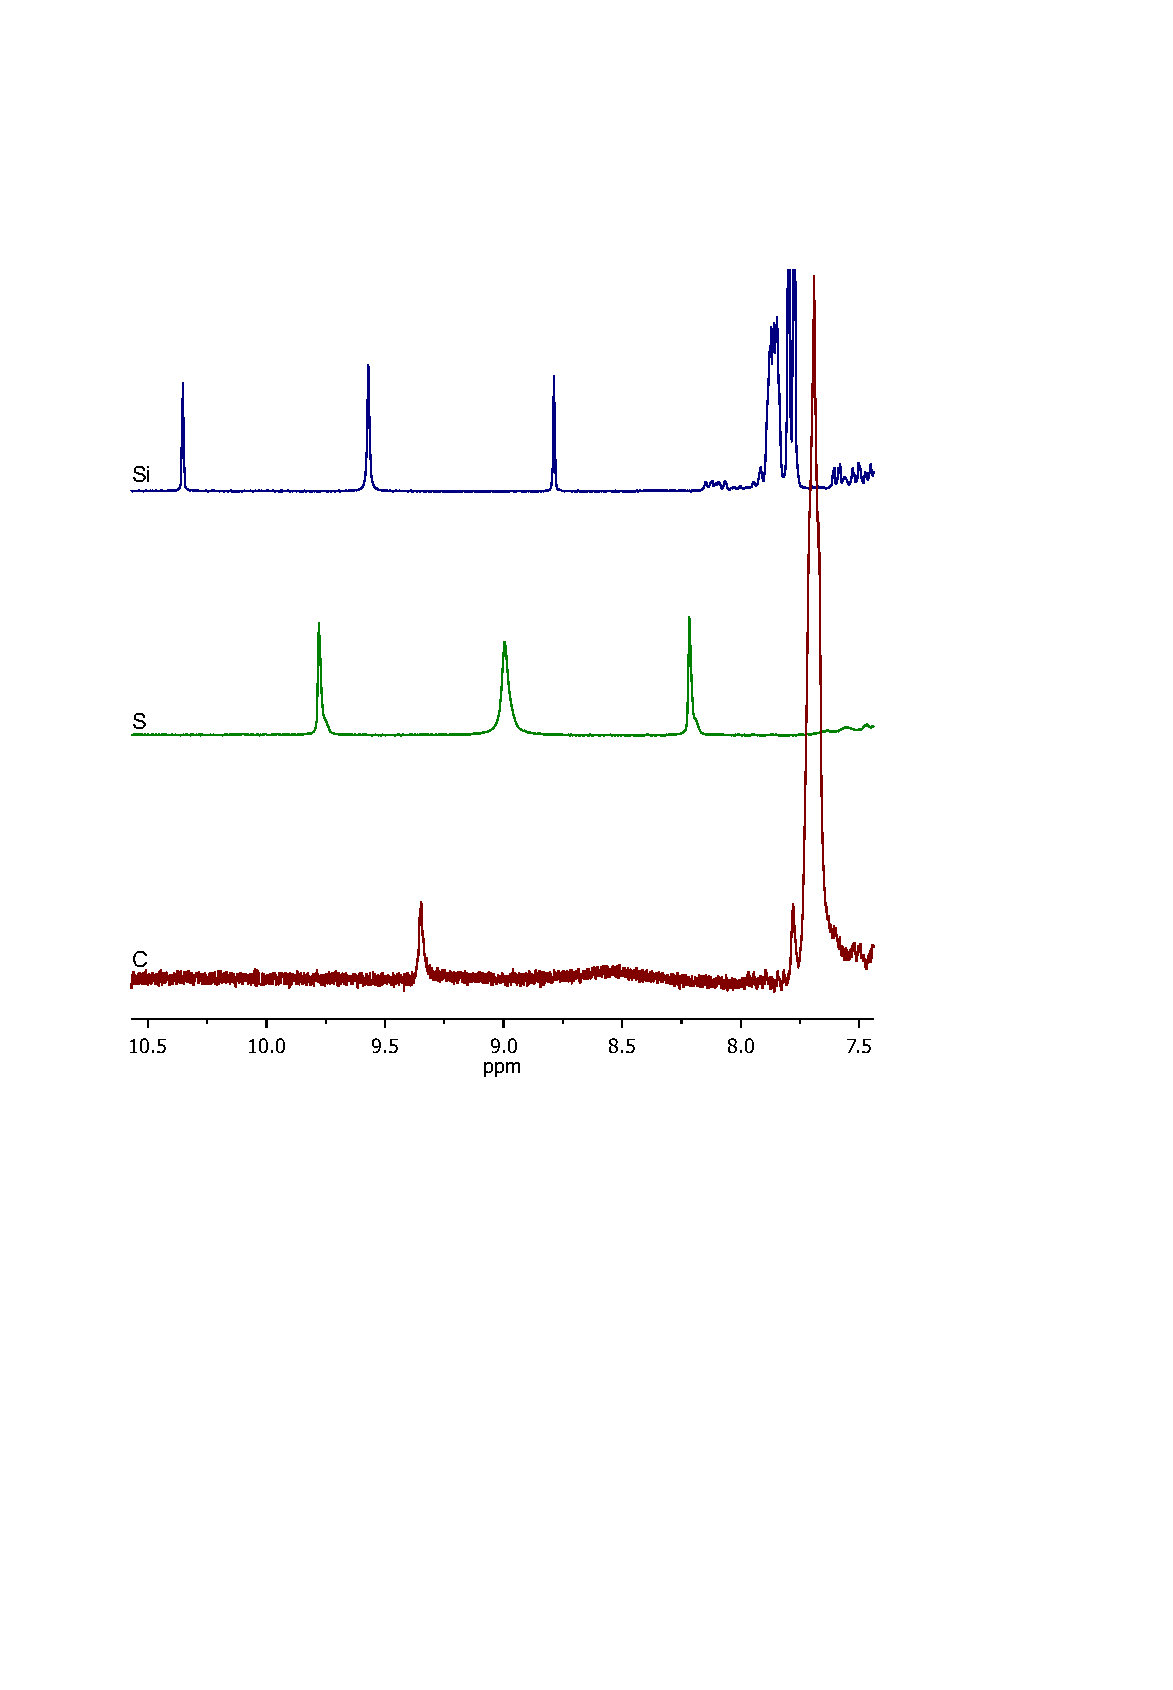
\includegraphics[scale = 0.8, trim = 1.5cm 10cm 4.5cm 5cm, clip]{../NMR/Phosphoniumstacked.eps}
\caption[\proton{} NMR spectra for \tBusixantphos, \tButhixantphos{} and \tBuxantphos{} showing the P-H region]{\proton{} NMR spectra in \ce{CDCl3} at 20\degC{} for \tBusixantphos, \tButhixantphos{} and \tBuxantphos{} (Si, S and C respectively) showing the P-H region}
\vspace{0.2cm}
\label{Protonatedligandsnmr}
\end{center}
\end{figure}
\vspace{0.2cm}


%\begin{figure}[htp]
%\begin{center}
%\vspace{0.5cm}
%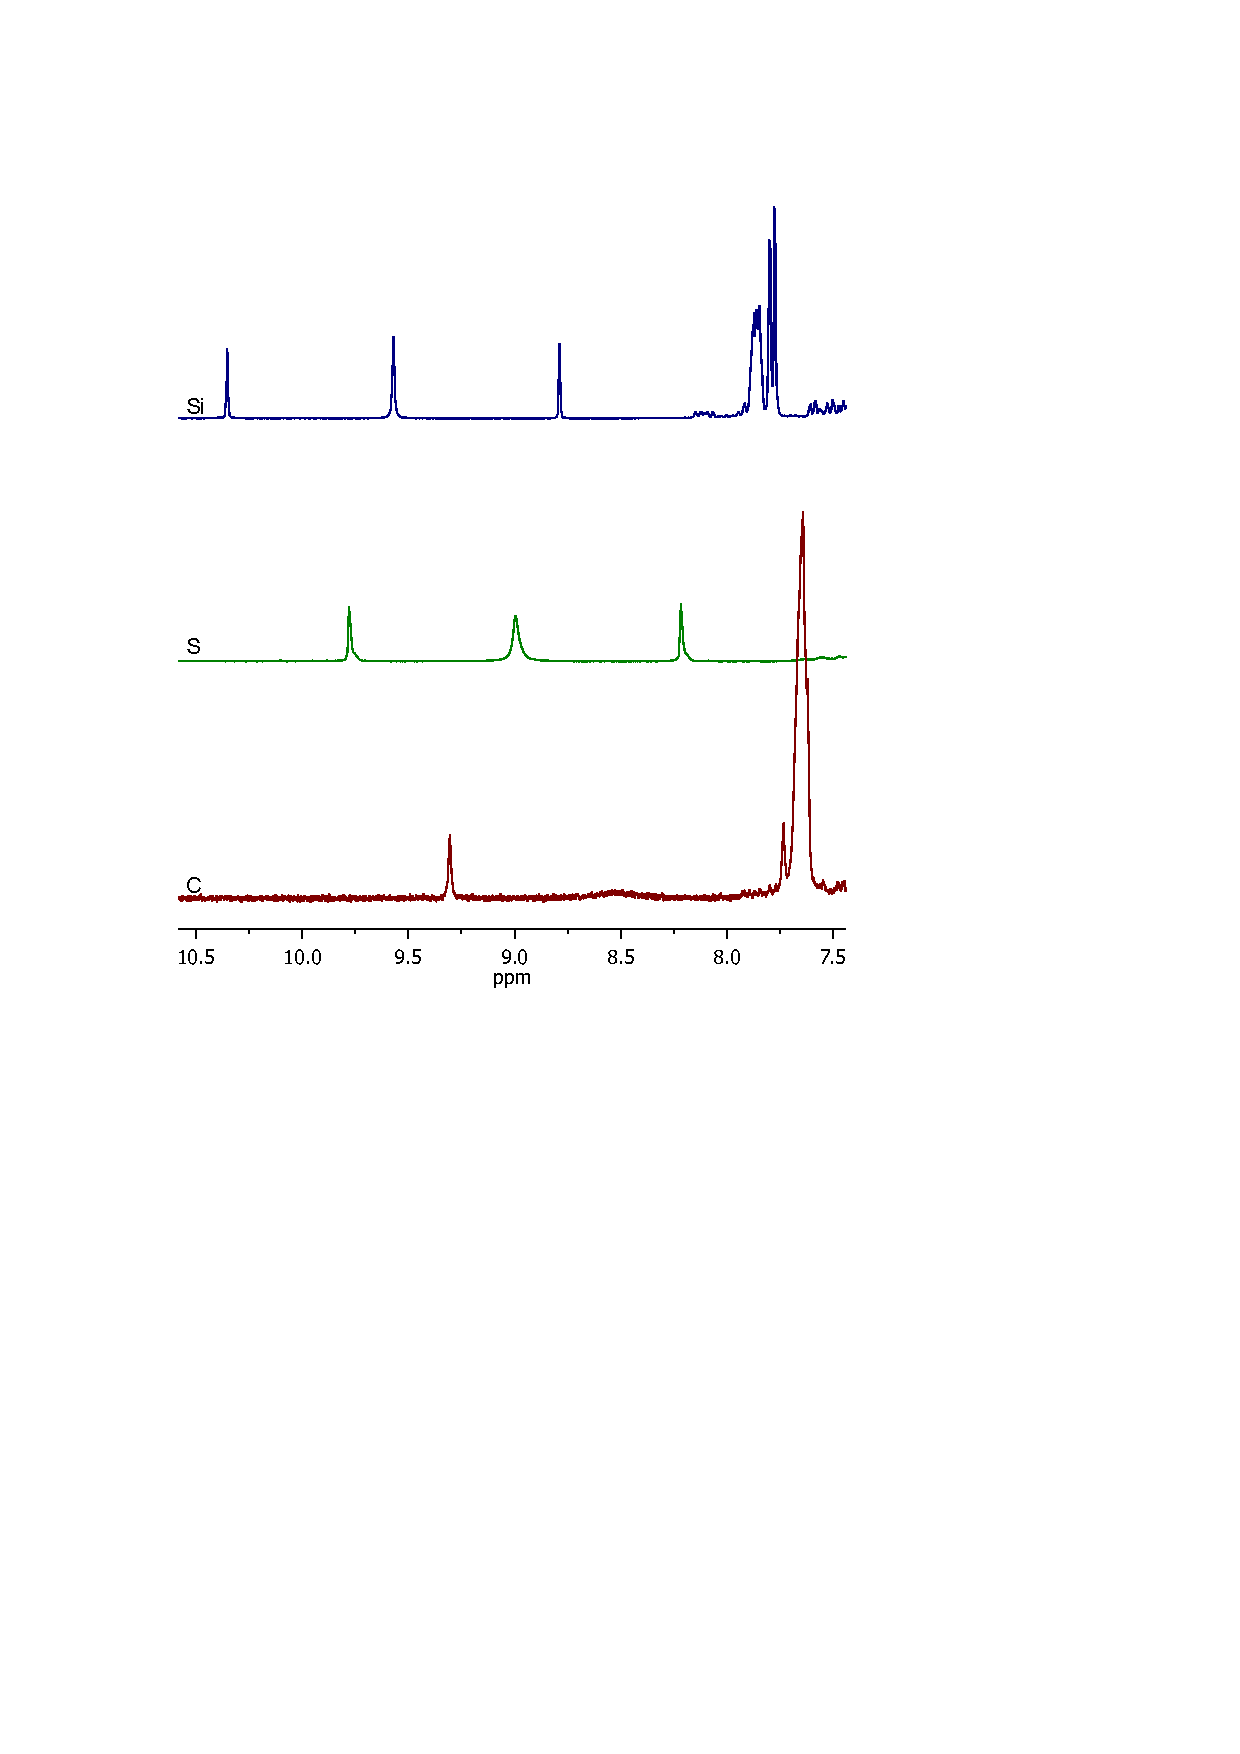
\includegraphics[scale=0.85]{../Figures/VTNMR/Protonatedligands.pdf}
%\caption[\proton{} NMR spectra for \tBusixantphos, \tButhixantphos{} and \tBuxantphos{} showing the P-H region]{\proton{} NMR spectra in \ce{CDCl3} at 20\degC{} for \tBusixantphos, \tButhixantphos{} and \tBuxantphos{} (Si, S and C respectively) showing the P-H region}
%\vspace{0.2cm}
%\label{Protonatedligandsnmr}
%\end{center}
%\end{figure}
%\vspace{0.2cm}

The dynamic behaviour of the phosphonium ions was further investigated using variable temperature \phosphorus{} and \proton{} NMR experiments on [(\tButhixantphos)H]\ce{CH(SO2CF3)2} (Figure \ref{VTStBuH})  At room temperature a single peak is present in the \phosphorus{} NMR spectrum.  When heated this peak shifts slightly to higher ppm and becomes sharper.  This single peak indicates that the exchange of the proton between the two phosphorus atoms is occurs rapidly enough that the two phosphorus atoms appear to have the same environment on the NMR timescale.  Cooling below room temperature causes the singlet to broaden significantly with coalescence occurring around -40\degC{}.  At -60\degC{} two signals are present though they are still broad.  One of these signals resolves into a clear doublet at -80\degC, however the other peak is still very broad ranging from 11-23 ppm.  Given the chemical shift of the free ligand it is likely that the sharp doublet belongs to the unprotonated phosphorus and the broad peak correlated with the protonated phosphorus.  This is also consistent with the shift of the peaks at higher temperature where we observe a shift to higher ppm as the rate of exchange is increased.  

\begin{figure}[h!]
\begin{center}
\vspace{0.5cm}
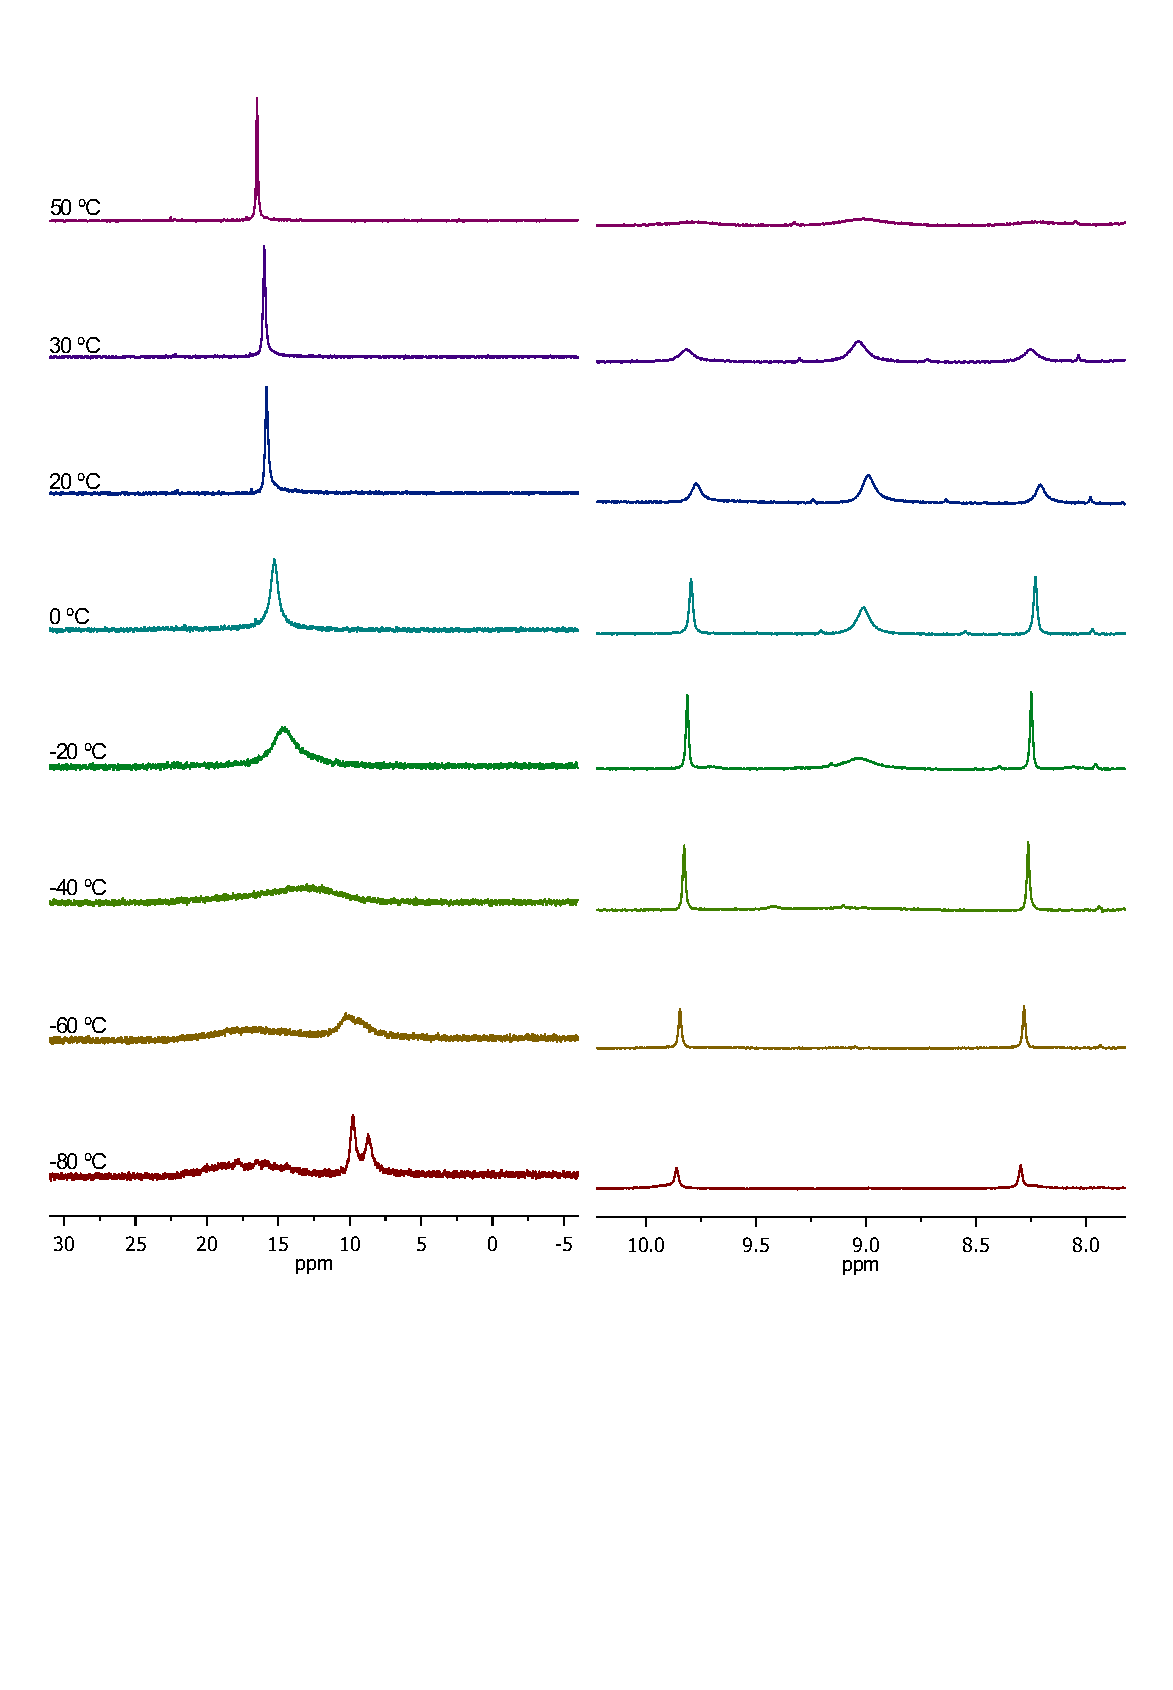
\includegraphics[scale=0.8, trim = 0cm 6.8cm 0cm 2cm]{../NMR/PhosphoniumVTNMRboth.eps}
\caption[Variable temperature \phosphorus{} and \proton{} NMR data for {[}(\tButhixantphos)H{]}\ce{CH(SO2CF3)2}]{Variable temperature \phosphorus{} (right) and \proton{} (left) NMR data for [(\tButhixantphos)H]\ce{CH(SO2CF3)2}}
\vspace{0.2cm}
\label{VTStBuH}
\end{center}
\end{figure}
\vspace{0.2cm}

%\begin{figure}[h!]
%\begin{center}
%\vspace{0.5cm}
%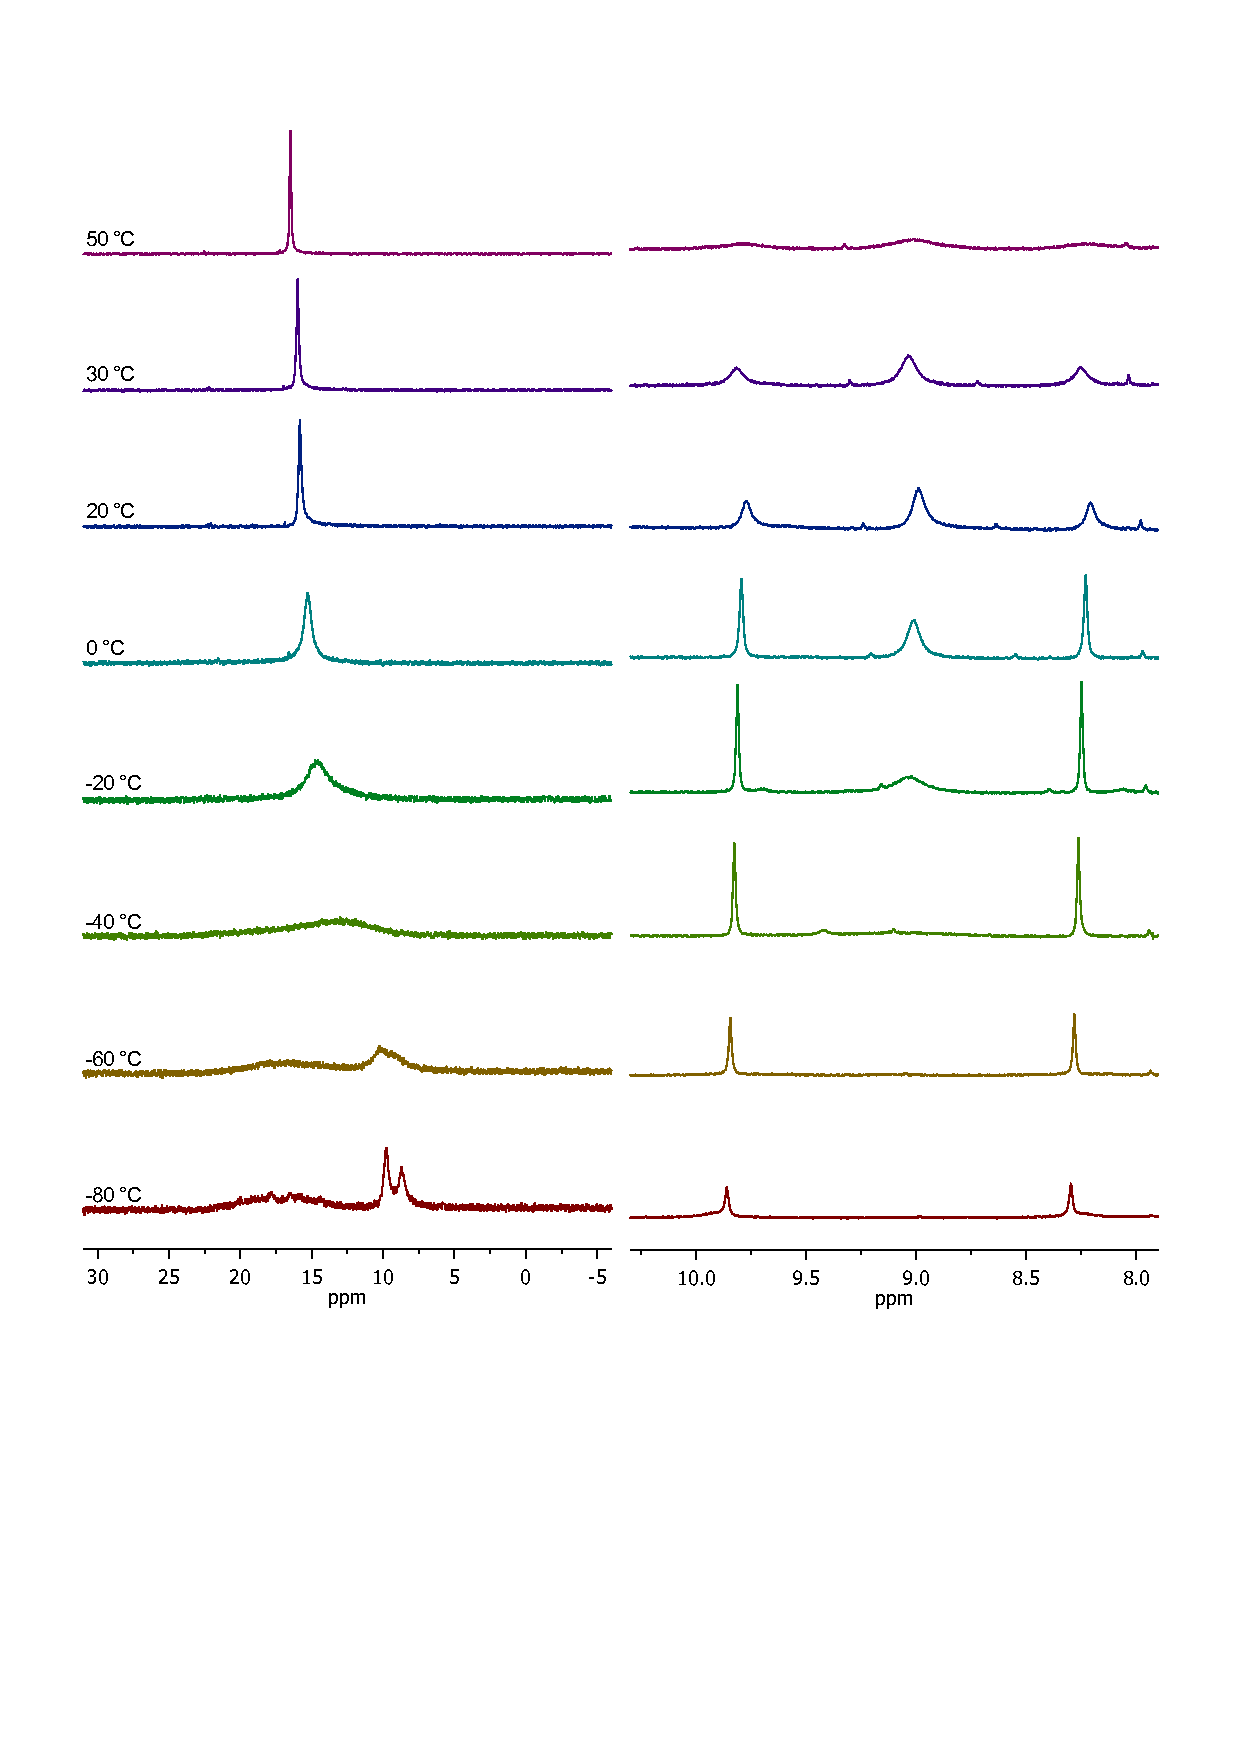
\includegraphics[scale=0.8]{../Figures/VTNMR/StBuHboth.pdf}
%\caption[Variable temperature \phosphorus{} and \proton{} NMR data for {[}(\tButhixantphos)H{]}\ce{CH(SO2CF3)2}]{Variable temperature \phosphorus{} (right) and \proton{} (left) NMR data for [(\tButhixantphos)H]\ce{CH(SO2CF3)2}}
%\vspace{0.2cm}
%\label{VTStBuH}
%\end{center}
%\end{figure}
%\vspace{0.2cm}

The variable temperature \proton{} NMR data for [\tButhixantphos\ce{H]CH(SO2CF3)2} (Figure \ref{VTStBuH}) shows a similar effects as the \phosphorus{} NMR spectra.  At low temperature the proton is static on a single phosphorus atom so we observe a doublet.  As the temperature increase to -20 \degC{} we observe a broad signal appearing in the centre of the doublet as exchange begins to occur and the signal changes from a simple double to a XAA'X' spin system.  This signal increases and at 20 \degC{} all three peaks begin to broaden again with coalescence at 50 \degC. This broadening which has a coalscence at around 50 \degC{} is the result of the proton no longer being isolated on a single molecule but delocalised across the entire system.   

Typically \phosphorus{} NMR spectra are proton decoupled.  However, with very strongly coupled systems such as phosphonium ions the decoupler is not able to fully decouple the spin system resulting in broadening and side bands.  To further investigate the [\tButhixantphos\ce{H]CH(SO2CF3)2} system proton coupled phosphorus NMR spectra were obtained at room temperature and -80\degC{} (Figure \ref{VTStBuHcoupled}).  At room temperature a simple doublet appears as expected.  This indicates rapid movement of the proton between the two phosphorus atoms.  When cooled to -80\degC{} the \phosphorus\{\proton\} spectrum showed a doublet and a broad singlet.  In the proton coupled phosphorus spectrum the doublet is retained confirming that this is the non-protonated phosphorus showing coupling to the protonated phosphorus.  The broad singlet resolves into a doublet of doublets with coupling constants consistent with coupling to the proton and the other phosphorus.  This further confirms that no exchange of the proton is occurring at low temperature.  

\begin{figure}[htp]
\begin{center}
\vspace{0.5cm}
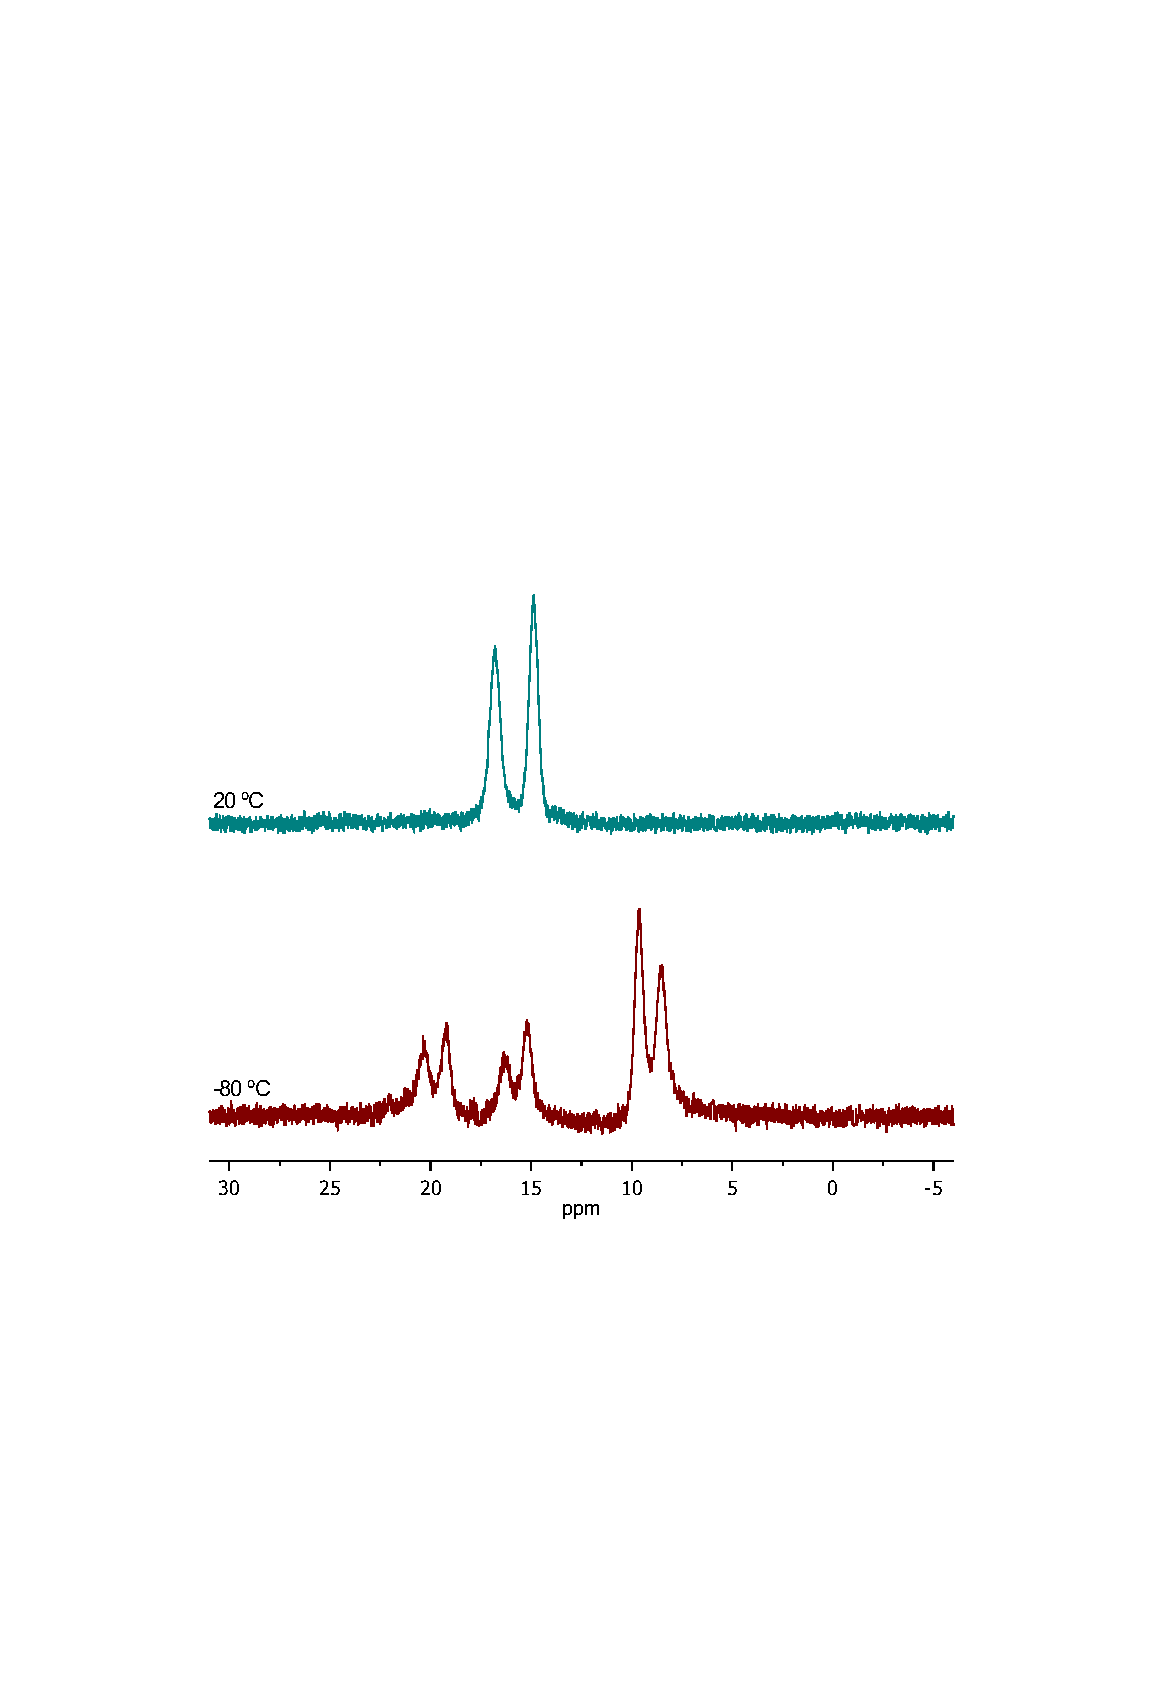
\includegraphics[scale = 0.8, trim = 0cm 8cm 0.5cm 10cm, clip]{../NMR/Coupledstacked.eps}
\caption[Variable temperature proton coupled \phosphorus{} NMR spectra for (\tButhixantphos)H+]{Variable temperature proton coupled \phosphorus{} NMR data for (\tButhixantphos)H+}
\vspace{0.2cm}
\label{VTStBuHcoupled}
\end{center}
\end{figure}  
\vspace{0.2cm}


%\begin{figure}[htp]
%\begin{center}
%\vspace{0.5cm}
%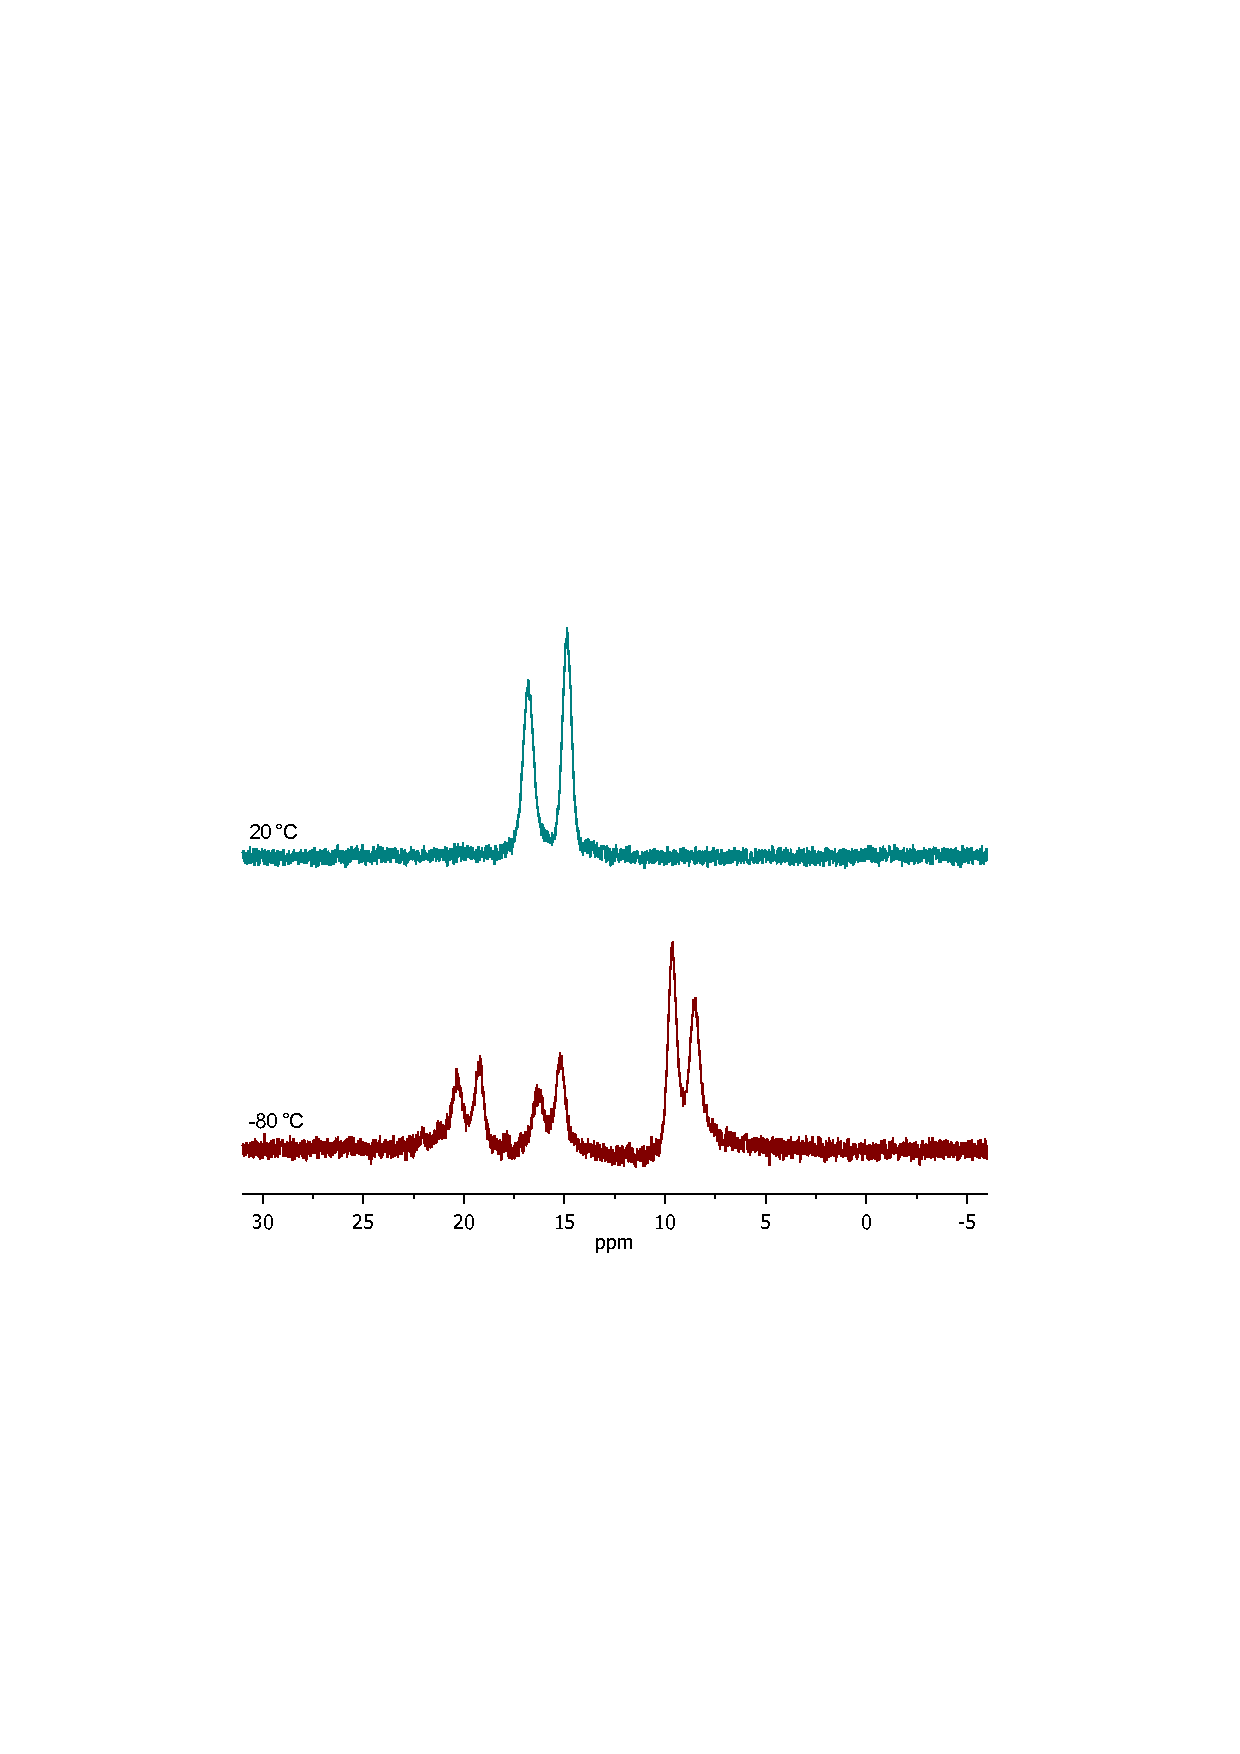
\includegraphics[scale=0.8]{../Figures/VTNMR/StBuHcoupled.pdf}
%\caption[Variable temperature proton coupled \phosphorus{} NMR spectra for (\tButhixantphos)H+]{Variable temperature proton coupled \phosphorus{} NMR data for (\tButhixantphos)H+}
%\vspace{0.2cm}
%\label{VTStBuHcoupled}
%\end{center}
%\end{figure}  
%\vspace{0.2cm}

%The protonation of the ligands was carried out using either or .  These are both strong acids with \pKa s of 2.0 and 2.4 in DMSO.\cite{Koppel2000}  The direct protonation of the ligands using a strong acid resulted in the phosphonium ions shown in Scheme \ref{Protonation}. 

%The degree of dynamism changes between the three ligands.  The sulfur bridged ligand with the smallest \biteangle{} has the greatest degree of exchange between the systems \fixme{can I get temperatures for coalescence as this would prove it nicely}.  \fixme{the S has the middle one need to check how much coupling in the carbon one}  The sulfur bridged ligand has very little coupling evident in the NMR spectra compared to the silicon bridged ligand which has a number of clearly defined coupled peaks.  The silicon bridged ligand has the largest degree of exchange at room temperature as the phosphorus atoms are held much closer - as shown by the smaller \biteangle{} which would indicate a greater degree of interaction between the tertiary phosphine and the phosphonium ion and thus much more rapid exchange.  As such at room temperature we are below coalescence and thus the NMR peaks resolve into much clearer signals than those found with the sulfur or carbon bridged systems.

%Likewise the carbon bridged system with the largest \biteangle{} will have the smallest degree of exchange at room temperature.  Hence we are closer to coalescence than in the other two so the NMR spectra are very broad and unable to be fully assigned.  \fixme{check the NMR data for 3013 on 600 MHz}

%Variable temperature phosphorus and proton NMR data for is shown in Figures \ref{VTStBuHphosphorus} and \ref{VTStBuHproton}

Colourless crystals of \ce{2{[}StBu-xantphos(H){]}CPh(SO2CF3)2}$\cdot{}$ \ce{C6D6} suitable for X-ray diffraction were grown from the reaction mixture in benzene.  The compound crystallised with a benzene solvate, \ce{[StBu-xantphos(H)]CPh(SO2CF3)2}$\cdot{}$ \nicefrac{1}{2}\ce{C6D6} in the monoclinic space group \emph{P}2\sub{1}/\emph{n}.  Selected bond lengths and angles are summarised in Table \ref{table:crystalprotonated:lengths} and crystallographic data is given in Table \ref{table:crystalprotonated:data}.  Although the cationic portion was well refined there was significant disorder around one of the counterions.  The proton on the phosphonium ion was able to be located and is exclusively located on a single phosphorus atom.  As a result of this the estimated standard deviations (e.s.d's) on the bond lengths and angles involving this proton are relatively high.  The distances from the proton to the other phosphorus or to the oxygen atom are both too long to indicate any degree of interaction.  The crystal structure was collected at 284.87 K, based on the variable temperature NMR data we would expect significant exchange of the proton at this temperature.  However, this is not apparent in the X-ray structure indicating that the exchange does not occur in the solid state.  

\begin{figure}[hp!]
\begin{center}
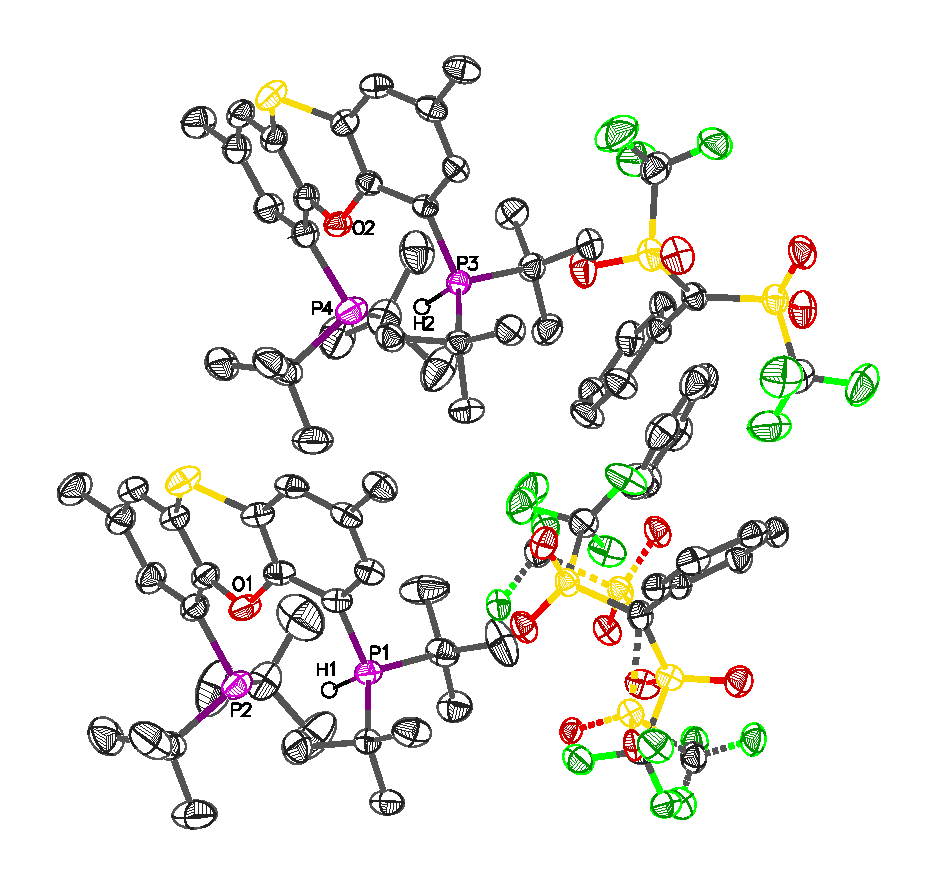
\includegraphics{../Crystalstructures/mrmnb.eps}
\caption[X-ray crystal structure of \ce{{[}StBu-xantphos(H){]}CPh(SO2CF3)2}]{X-ray crystal structure of \ce{2{[}StBu-xantphos(H){]}CPh(SO2CF3)2}$\cdot{}$ \ce{C6D6} (50\% probability thermal ellipsoids).  Selected hydrogen atoms omitted for clarity}
\label{Crystalprotonated}
\end{center}
\end{figure}

\begin{table}[htp]
\small
\caption[Selected bond distances (\AA) and angles (\degrees) of \ce{StBu-xantphos(H)]CPh(SO2CF3)2}$\cdot{}$ \nicefrac{1}{2}\ce{C6D6}]{Selected bond distances (\AA) and angles (\degrees) of \ce{StBu-xantphos(H)]CPh(SO2CF3)2}$\cdot{}$ \nicefrac{1}{2}\ce{C6D6}} 
\vspace{1em}
\label{table:crystalprotonated:lengths}
\begin{center}
\begin{tabular}{l l l l l}
	\toprule
	\multicolumn{2}{l}{\bfseries{~Bond distances (\si{\angstrom})}} &~~~& \multicolumn{2}{l}{\bfseries{Bond angles (\degrees)}} \\
	\midrule		
	P1-H1	& 1.22(3)		&~~~& P1-H1...P2	& 160(2)\\
	P2...H1	& 2.96(3)		&~~~& P1...O1...P2	& 89.19(6)\\
	P1...P2	& 4.1290(11)	&~~~& P3-H2...P4	& 154(2)\\
	O1...H1	& 2.44(3)		&~~~& P3...O2...P4	& 86.40(5)\\
	P3-H2	& 1.22(3)		&~~~& Ring 1...Ring 2 & 18.28(10)\\
	P4...H2	& 2.91(3)		&~~~& Ring 3...Ring 4 & 26.67(10)\\
	P3...P4	& 4.0372(11)	&~~~& ~			& ~\\
	O2...H2	& 2.43(3)		&~~~& ~			& ~\\
	\bottomrule{}
\end{tabular}
\end{center}
\end{table}

\begin{table}[htp]
\small
\caption[Crystallographic Data and Structure Refinement of \ce{2[StBu-xantphos(H)]CPh(SO2CF3)2}$\cdot{}$\ce{C6D6}]{Crystallographic data of \ce{2[StBu-xantphos(H)]CPh(SO2CF3)2}$\cdot{}$
\ce{C6D6}} 
\vspace{1em}
\label{table:crystalprotonated:data}
\small
\begin{center}
\begin{tabular}{l l}
	\toprule
	\bfseries{Empirical formula}~~& \bfseries{\ce{C84H110F12O10P4S6}}\\
	\midrule
	Formula weight	 							& 1823.95\\
	Temperature/K	 							& 284.87(10)\\
	Crystal system	 							& monoclinic\\
	Space group	 							& P21/n\\
	a$/$\si{\angstrom}							& 14.19615(12)\\
	b$/$\si{\angstrom} 							& 39.4563(3)\\
	c$/$\si{\angstrom}							& 16.35832(15)\\
	$\alpha/$\degrees							& 90\\
	$\beta/$\degrees							& 100.1751(8)\\
	$\gamma/$\degrees							& 90\\
	Volume$/$\si{\angstrom\cubed}  				& 9018.64(13)\\
	Z	 									& 4\\
$\rho$\sub{calc} \si{\milli\gram}$/$\si{\milli\metre\cubed} 	& 1.343\\
\si{\metre}$/$\si{\milli\metre} 							& 2.749\\
F(000)	 									& 3832.0\\
Crystal size$/$\si{\milli\metre\cubed}	 				& \fixme{? � ? � ?}\\
Radiation	 									& CuK$\alpha$ ($\lambda$ = 1.54184)\\
2$\theta$ range for data collection					& 5.928 to 147.832\degrees\\
Index ranges	 								& -17 $\leq$ h $\leq$ 17, -48 $\leq$ k $\leq$ 48, -20 $\leq$ l $\leq$ 20\\
Reflections collected	 							& 69203\\
Independent reflections	 						& 17960 [R\sub{int} = 0.0261, R\sub{sigma} = 0.0219]\\
Data$/$restraints$/$parameters					& 17960$/$291$/$1221\\
Goodness-of-fit on F$^{2}$	 					& 1.068\\
Final R indexes [I$>$=2$\sigma$ (I)]	 				& R\sub{1} = 0.0549, wR\sub{2} = 0.1473\\
Final R indexes [all data]	 						& R\sub{1} = 0.0623, wR\sub{2} = 0.1531\\
Largest diff. peak/hole / e \si{\per\angstrom\cubed}		& 1.11/-0.56	\\
	\bottomrule
\end{tabular}
\end{center}
\end{table}

\section{Selenides}
\label{section:selenides}

Numerous approaches to studying the steric influence of phosphine and diphosphine ligands exist, the most prolific are the Tolman cone angle\cite{Tolman1977} and the natural bite-angle\cite{Casey1990}.  The electronic influence are less well defined, typical approaches involve the CO stretching frequency of metal carbonyl complexes or analysis of \oneJPM{} spin-spin coupling constants.  However, the coupling constants are highly dependent on the geometries of metal complexes and this can be influenced significantly be steric constraints, such as those imposed by large diphosphine ligands.  As such the \JPSe{} spin-spin coupling constants of the phosphine selenides is often used as a more accurate measure of the electronic properties of tertiary phosphines.\cite{Beckmann2011} In this case the more electron donating the phosphorus substituents are, the lower the resulting \JPSe{}.  

The \JPSe{} coupling constant has shown to correlate relatively well with the Tolman electronic parameter.\cite{Allman1982}  Further the phosphino-selenides are generally relatively straightforward to synthesise by reaction of the phosphine with either elemental selenium or potassium selenocyanide (with or without heating).\cite{Beckmann2011}  Using the phosphino-selenides to investigate the electronic properties of the phosphine also avoids the expensive transition metals used in other methods.  In addition the resulting phosphino-selenides are air-stable as compared to metal carbonyl complexes which often decompose if not stored under carbon monoxide.   Further if elemental selenium is utilised then the use of toxic gases is avoided (not the case for potassium selenocyanide which produces potassium cyanide as a by-product which will react rapidly with any proton source to form hydrogen cyanide).  

Phosphorus-selenium coupling constants are not without their restrictions, particularly with diphosphines.  It is not possible to completely eliminate steric influences on the \JPSe{}, selenium has a significant steric and electronic impact resulting in repulsion of the two phosphino-selenides.  This has been noted as the mono- and di-selenides of diphosphines often have different coupling constants.  In these cases the mono-selenide generally gives a better description of the electronic influence of the diphosphine.  

In addition to the use of \JPSe{} as a measure of the electronic influence of a phosphine it can also be used to measure the Br\o{}nsted basicity of a given phosphine.  A correlation between the experimentally measured \pKb{} and the \JPSe{} has been reported\cite{Beckmann2011} with linear regression: \JPSe{}$ = 7.60 \times{} $ \pKb{} $~+~646~($R$_{2} = 0.9492)$.  As such determining the \JPSe{} allows for calculation of the \pKb{} and has shown good agreement with the experimentally determined data.  One significant limitation of this method is the significant impact that sterically bulky groups can have.  For \ce{PtBu3} the correlation suggests a \pKb{} value of 6.0 however the experimentally determined value is 2.60.\cite{Beckmann2011}  This is the result of the \tBu{} groups increasing the C-P-C angles, thus decreasing the s-character of the lone pair.

The ligands \fixme{compound references} showed significant resistance to selenation.  Typical methods include heating the phosphine with elemental selenium or reacting with KSeCN.\cite{Muller2008c}  Reaction directly with elemental selenium has been reported as preferable to potassium selenocyanide as the later reacts slowly and gives lower yields.\cite{Beckmann2011}  The previously reported \Phxantphos{} selenide was synthesised by refluxing \Phxantphos{} and red selenium in toluene overnight resulting in diselenation.  Attempting this method with the \tBuxantphos{} ligands reported here showed little reaction.  Attempts were also made using KSeCN similar to those previously reported \cite{Bungu2007}.  However, these were also unsuccessful.  Successful monoselenation was obtained by refluxing the ligands with a large excess of grey selenium in toluene for 3 days (Scheme \ref{Selenation}).  Extending the reaction period did not result in the formation of any diselenide.  This is likely due to the steric restraints of these ligands.

\begin{scheme}[hp!]
\begin{center}
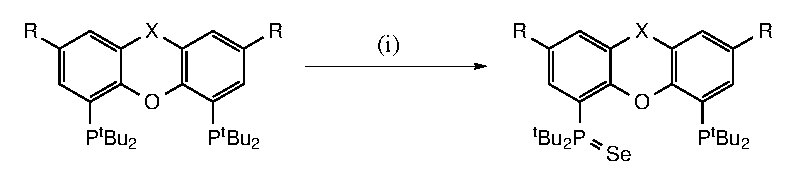
\includegraphics{../Schemes/Selenation.eps}
\caption[Selenation of \tBuxantphos{} ligands]{Selenation of \tBuxantphos{} (X = \ce{CMe2}, R = H), \tButhixantphos{} (X = S, R = Me) and \tBusixantphos{} (X = \ce{SiMe2}, R = H).}
\label{Selenation}
\end{center}
\end{scheme}

The \phosphorus{} NMR spectra of the three phosphino-selenides showed significant differences.  For \tBuxantphos{}selenide two clear peaks were observed in a 1:1 ratio clearly indicating the formation of the monoselenide.  For \tButhixantphos{} and \tBusixantphos{} multiple peaks were observed though only one in the region expected for an non-selenated phosphine.  There were two moderately broad peaks at higher ppm close to where the selenated phosphorus of \tBuxantphos{}selenide appeared.  Variable temperature \phosphorus{} NMR showed that the ratio of these peaks changed at low temperature \fixme{add the spectra} leading us to propose the presence of two distinct rotamers.  

These rotomers were investigated using density functional theory (DFT) using the B3LYP functional and TZVP basis set.  Two rotamers (representative structures shown for \tButhixantphos{} shown in Figure \ref{Seleniderotomers} were found as minima for all three ligands, with very close energy values thus indicating little difference between the two.  However, it is likely the a significant barrier to interconversion exists due to the steric restraints of the system.  

% The \JPSe{} values vary across a range of 12 Hz.  The \JPSe{} values for \tBuxantphos{} and \tButhixantphos{} are similar, with a difference of 1.4 Hz; whilst \tBusixantphos{} has a much smaller \JPSe{} value (Table \ref{table:selenides}).  

The NMR data for the major rotamer is summarised in Table \ref{table:selenides}.  The \JPSe{} values are similar for the three ligands with a range of 12 Hz.  The monoselenated \tButhixantphos{} derivative was found to have a \JPSe{} = 698.5 Hz, while the monoselenated \tBuxantphos{} has a \JPSe{} = 696.3 Hz.  These are much lower than that reported for xantphos selenide (749 Hz)\cite{Jahromi2012}.  This lower coupling constant is expected as \emph{tert}-butyl groups are more electron donating than phenyl substituents.  Data for the monoselenated \tBuxantphos{} derivatives are summarised in Table \ref{table:selenides}.  Upon monoselenation a signal for one of the aromatic protons shifts from 7.60 to 9.26 ppm.   This is likely the proton adjacent to the selected phosphorus as the proximity to the selenium will reduce the shielding on the proton resulting in a downfield chemical shift.

\begin{table}[ht]
\caption[NMR Data for Selenides]{NMR Data for Selenides}
\vspace{1em}
\label{table:selenides}
\small
\begin{center}
\begin{tabular}{l l l l}
	\toprule
	\bfseries{Diphosphine} & \bfseries{\phosphorus (P, P=Se ppm)} & \bfseries{\JPSe (Hz)} & \bfseries{\pKb} \\
	\midrule		
	\tBuXantphos		&10.6, 101.9	&~697.1	&6.72	\\
	\tBuThixantphos	&11.7, 103.7	&~698.5	&6.90	\\
	\tBuSixantphos		&15.9, 102.7	&~689.1	&5.67	\\
	\bottomrule{}
\end{tabular}
\end{center}
\end{table}

Using the correlation reported by Beckmann \emph{et al.} it is possible to convert the \JPSe{} of 698.5~Hz into a \pKb{} of 6.91.  This makes the ligand significantly more basic than \Phxantphos{} with a \pKb{} of 13.55.  This significant difference is expected as tert-butyl groups are strongly electron donating whilst phenyl substituents are electron withdrawing.\cite{Tolman1977}  This effect will dominate any other subtle effects that may arise due to \biteangle and steric considerations.  

The determined \pKb{} values fall somewhere between those for \ce{PPhMe2} (experimental = 7.50, calculated = 8.4) and \ce{PMe3} (experimental = 5.35, calculated = 5.0)\cite{Beckmann2011}.  This is consistent with expectations as \tBu{} groups are more electron donating than methyl groups while the phenyl still results in a higher \pKb{} than those for the trialkyl phosphines.  

The bite-angle may play a role in the value for the \JPSe{} coupling constant as monoselenide diphosphines have shown through space coupling to the other phosphorus.\cite{Hierso2014}  This would result in a lower \JPSe{} value than otherwise expected and the effect would be more pronounced with smaller bite-angles.  In this case \tBusixantphos has the lowest \pKb{} of the three ligands and also the smallest bite-angle so a bite-angle effect may be present.  However, the differences cannot be purely the result of the bite-angle as \tButhixantphos{} has the largest \JPSe{} value but \tBuxantphos has the largest bite-angle.

In addition to the influence of the bite-angle on the \JPSe{} coupling constant there must exist another electronic effect contributing to the difference between the ligands.  Both \tButhixantphos{} and \tBuxantphos{} groups have an ortho ether and a meta alkyl group, in addition \tButhixantphos has the thioether bridge, thioethers are electron donating by resonance but being in the meta position to the phosphorus the negative charge that could be generated is unable to interact with the phosphorus.  With sulfur being slightly more electronegative than carbon, a thioether is also slightly inductively electron withdrawing which would result in the phosphorus being very slightly less basic in the \tButhixantphos{} case compared to the \tBuxantphos{}.

\section{Conclusions}


